\section{Toro}
\emph{Toro} has a complicated kinematic structure as shown in Figure \ref{fig:toro_kin}. It consists of 3 kinematic chains branching from the common base. The hip acts as the common base. The three chains branching from the hip are  upper body, right leg and left leg. The upper body further branches into right hand and left hand. The two arms and legs acts as the end effectors of \emph{Toro}.

\begin{figure}
\begin{center}
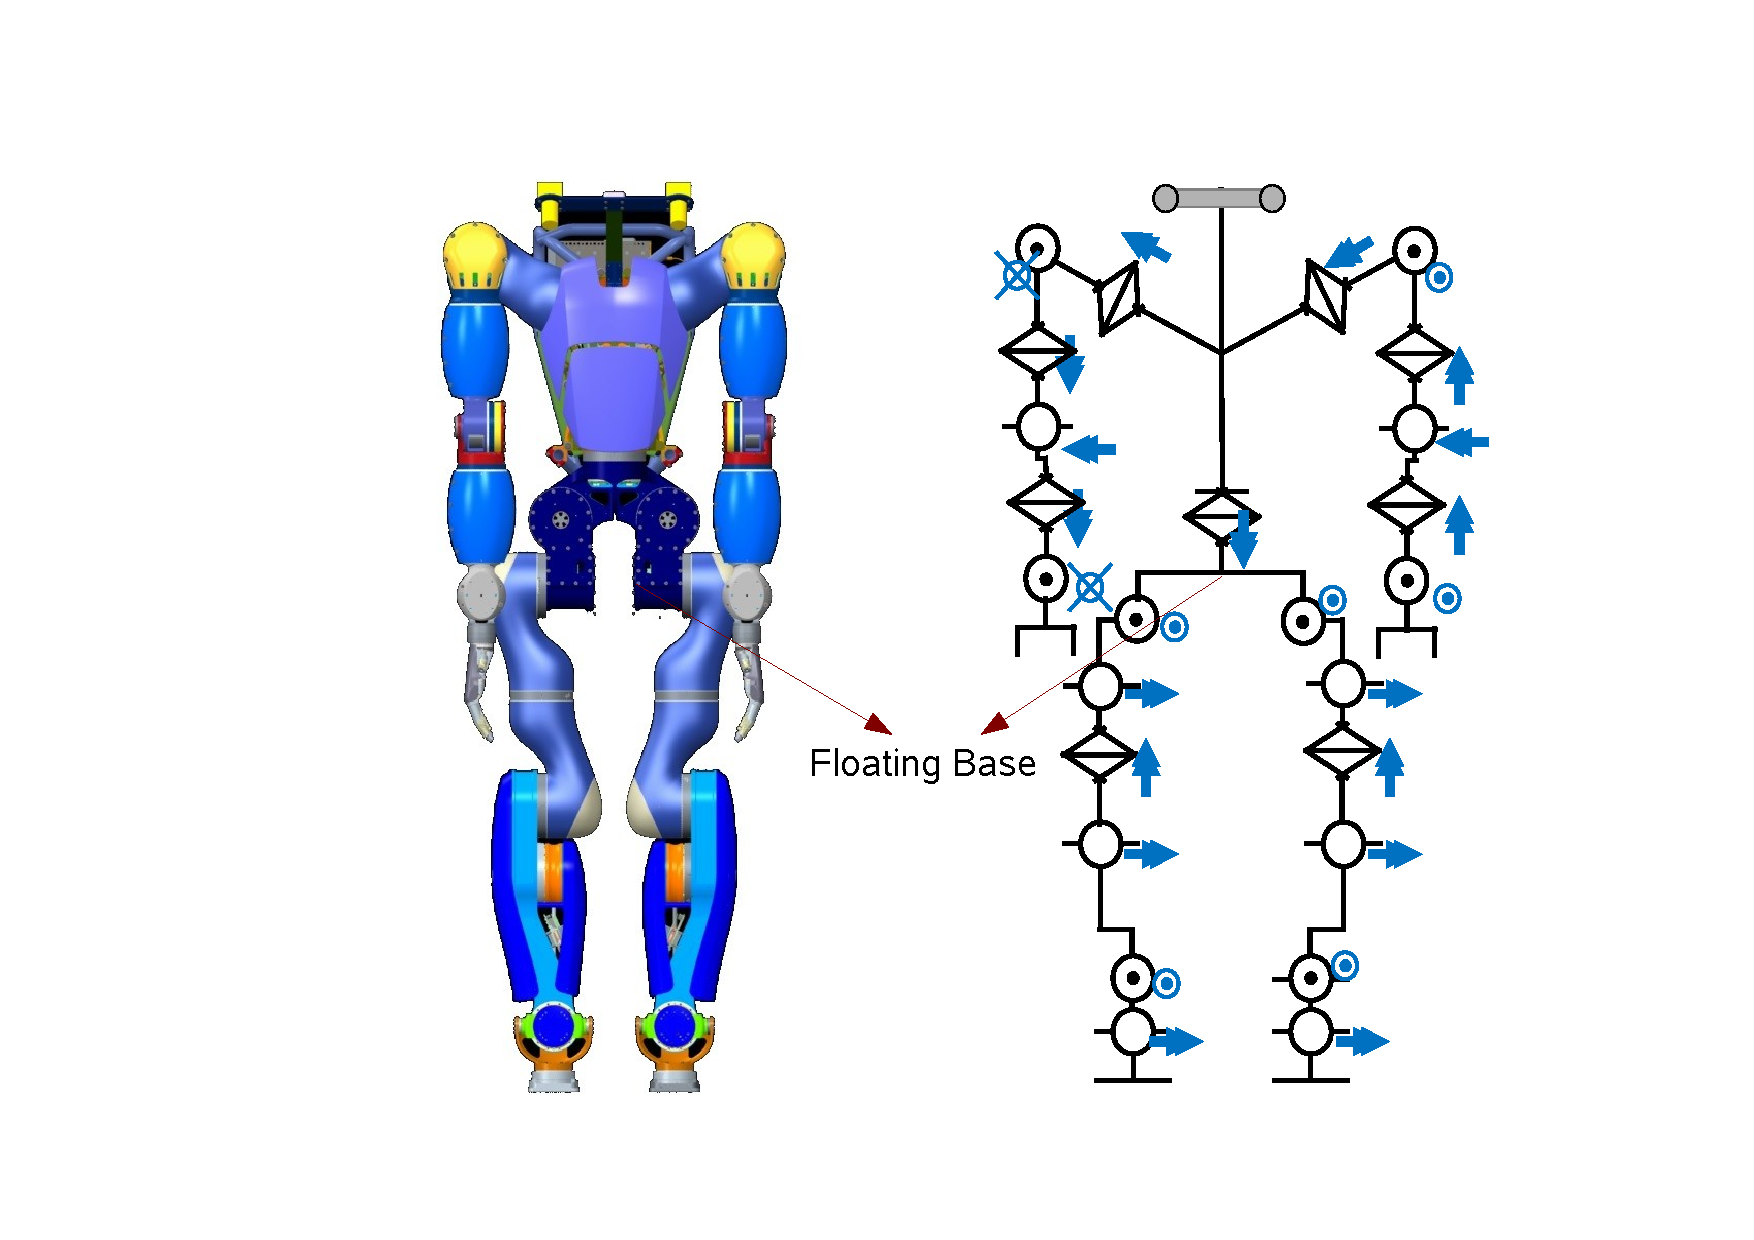
\includegraphics[trim= 70mm 10mm 40mm 10mm,clip,scale=0.7]{Bilder/TORO_kinematic.pdf}
\caption[Kinematic chain of \emph{Toro}]{Kinematic chain of \emph{Toro} \footnotemark }
\label{fig:toro_kin}
\end{center}
\end{figure}
\footnotetext{ The joint symbols are explained in Appendix \ref{fig:joint}.}
The generalized coordinates of \emph{Toro} are represented by a vector of joint angles $q$ and the coordinates of the base of robot $x^b$. The number of joints of a robot is the number of controllable degrees of freedom \cite[Chapter 2]{mur94}. The coordinates of the base $x^b$ are the under-actuated degrees of freedom of \emph{Toro}. 

A rigid body in space has six degrees of freedom as shown in Figure \ref{fig:rbody}.
%\begin{figure}
\begin{figure}
\begin{center}
%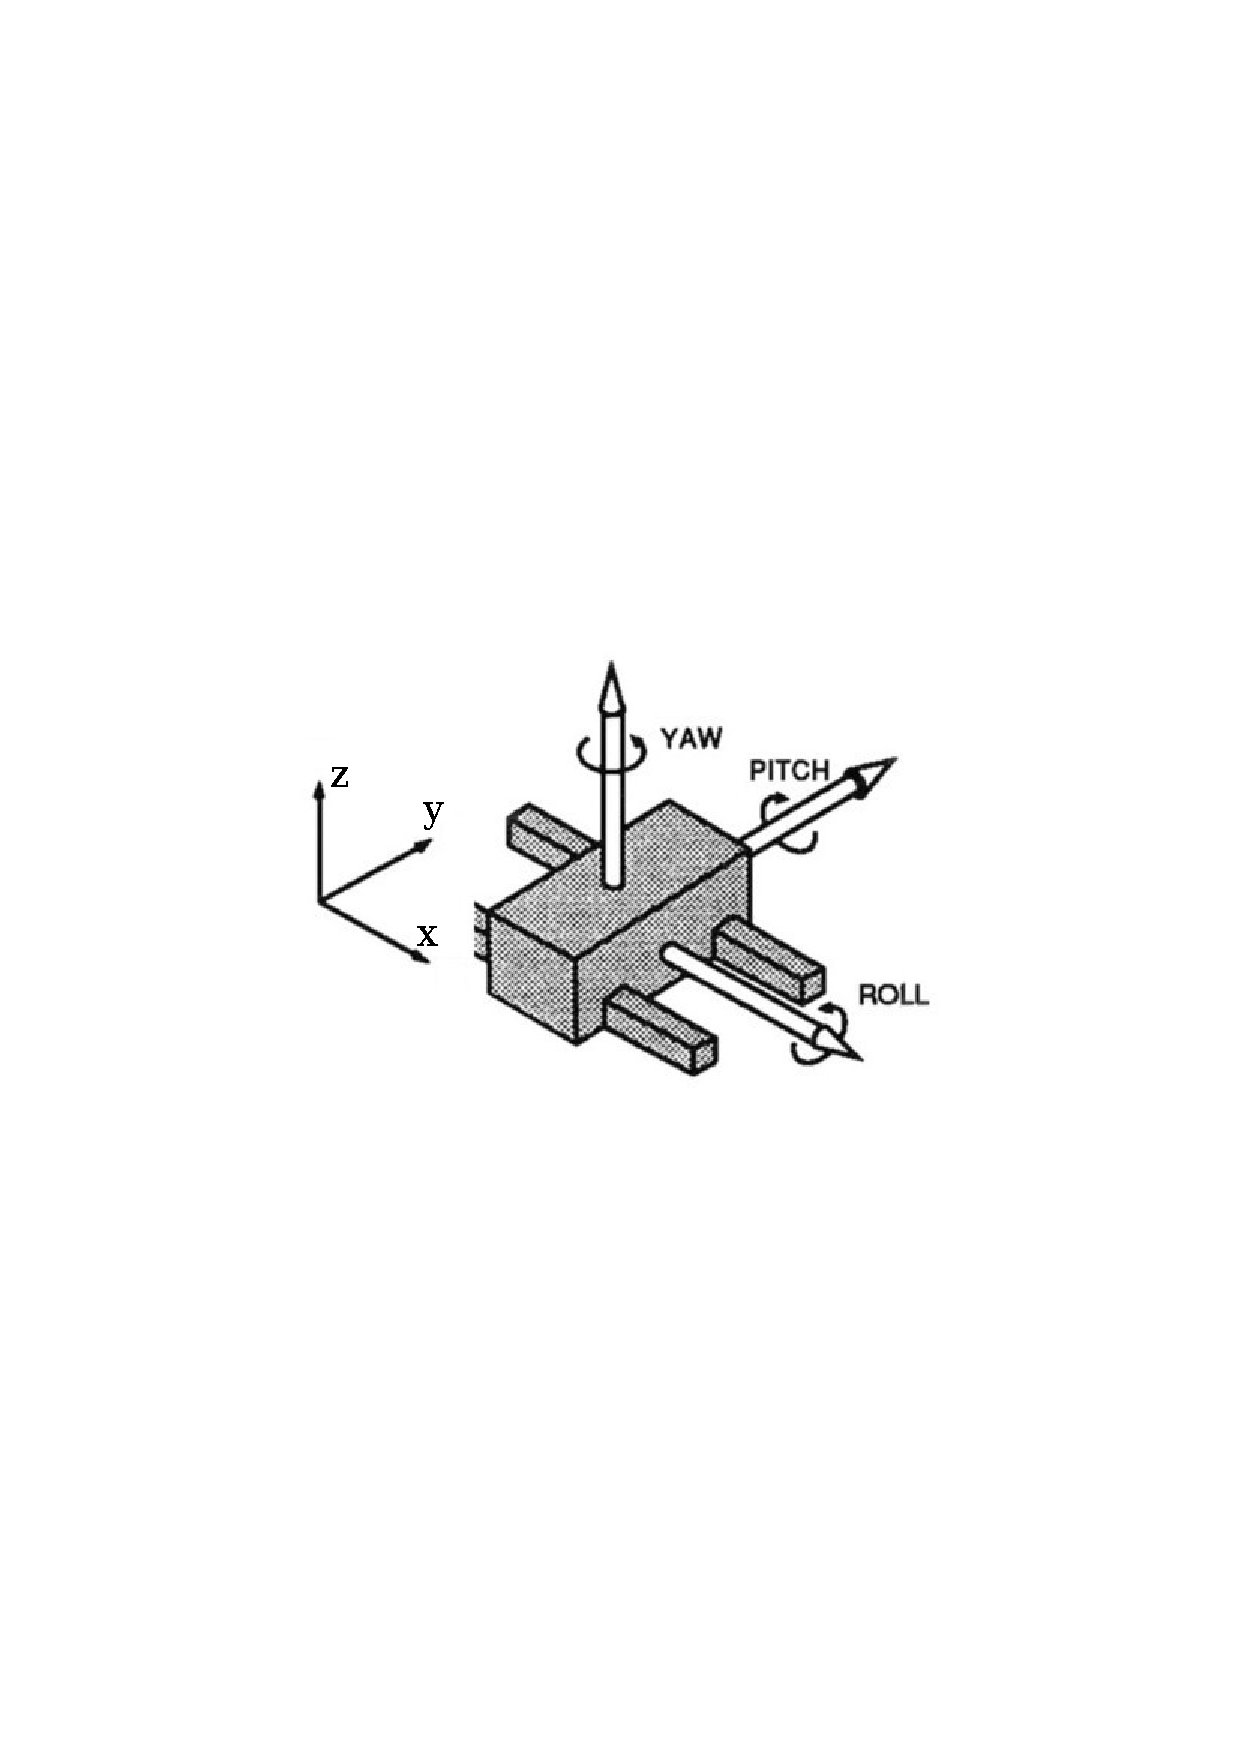
\includegraphics[trim= 30mm 100mm 10mm 120mm,scale=0.75]{Bilder/rbody_dof.pdf}
\begin{tikzpicture}[every node/.style={minimum size=1cm},on grid]
\begin{scope}[every node/.append style={yslant=-0.5},yslant=-0.5]
  \shade[right color=gray!10, left color=black!50] (0,0) rectangle +(3,3);
  \draw [->,line width=2pt] (1.5,1.5) --node {} (-3,-3) node[below]{};
  \draw (-2.4,-2.6)[yscale=1.3,->, line width=2pt] arc(-60:240:.25);
 \end{scope}
 \draw [|<->|] (0.5,-0.5) --node[below]{x} (-1.5,-1.5);
 \node (roll)[xshift=-2.5cm,yshift=-0.5cm] {Roll $\theta_x$};
 \node (xaxis) [below of=roll,node distance=1.5cm, xshift=-1cm]{\textbf{X}};
\begin{scope}[every node/.append style={yslant=0.5},yslant=0.5]
  \shade[right color=gray!70,left color=gray!10] (3,-3) rectangle +(3,3);
    \draw [->,,line width=2pt] (4.5,-1.5) --node {} (9.5,-6) ;
    \draw (8.5,-5.25) [yscale=1.3,->,line width=2pt]arc(-60:200:.25);
\end{scope}
	\node (yaxis) [xshift=9.5cm,yshift=-2cm] {\textbf{Y}};
	\node (pitch) [left of=yaxis, node distance = 1cm,yshift=2cm]{Pitch $\theta_y$};
	 \draw [|<->|] (5.5,-0.5) --node[below]{y} (7.5,-1.25);
\begin{scope}[every node/.append style={yslant=0.5,xslant=-1},yslant=0.5,xslant=-1]
  \shade[bottom color=gray!10, top color=black!80] (6,3) rectangle +(-3,-3);
  \draw [->,,line width=2pt] (4.5,1.5) --node {} (9,6) node[below]{};
  \draw (8,5) [yscale=1.3,->,line width=2pt]arc(30:280:.25);
\end{scope}
    \node (zaxis) [xshift=3.5cm,yshift=7.5cm]{\textbf{Z}};
    \node (pitch) [left of=zaxis, node distance = 2cm,yshift=-1cm]{Yaw $\theta_z$};
	\draw [|<->|] (	3.75,3.5) --node[right]{z} (3.75,6.25);
\end{tikzpicture}
\vspace{1cm}
\caption{Degrees of freedom of a rigid body }
\label{fig:rbody}
\end{center}
\end{figure}
The translational and rotational degrees of freedom of the rigid body in Figure \ref{fig:rbody} are \emph{x,y,z} and \emph{roll,pitch,yaw}. The rotational degrees of freedom \emph{roll,pitch,yaw} corresponds to rotation of the body around \textbf{X,Y,Z} axes. The base of \emph{Toro} is assumed to be a free rigid body. Since the base has all the six degrees of freedom which corresponds to degrees of freedom of rigid body floating in three dimensional space, it is called floating base. The equation of motion of a single rigid body(floating base) is given by Newton-Euler equation of motion in body coordinates \cite[Chapter 4]{mur94}:
%\footnotetext[1]{Image source:\url{http://www.cncexpo.com/Images/pitchyawroll.jpg}}
\begin{equation}
\label{eq:dyn_rig_bdy}
\begin{bmatrix}
mI_3 & \textbf{0}_3 \\ \textbf{0}_3 &\Im
\end{bmatrix}
\begin{bmatrix}
\dot{v}^b\\ \dot{\omega}^b
\end{bmatrix}
+ \begin{bmatrix}
\omega^b \times mv^b \\ 
\omega^b \times \Im w^b
\end{bmatrix}
= W.\\
\end{equation}
In the above equation, \emph{m} is the mass of the rigid body, $\Im$ is the moment of inertia of the rigid body. $I_3$ represents the $3 \times 3$ identity matrix and $ \textbf{0}_3$ represents the  $3 \times 3$ zero matrix. The translation velocity and angular velocity represented in body coordinate frame are ${v}^b$ and $\omega^b$. $W$ is the external wrench applied on the body. A wrench represents a force/moment pair. It is represented by vector in $\Re^6$ as \citep{mur94}
$$ W = \begin{bmatrix} F \\ \tau \end{bmatrix}, $$ where $F \in \Re^3$ is the linear component and $\tau \in \Re^3$ is the rotational component of the generalized force.

The external wrench $W$ acting on the body can be decomposed into wrench due to gravitational forces $g_x^b$ and wrench due to external forces $W^b$: $$ W = W^b - g_x^b.$$

To be consistent with the multibody system dynamics formulation in Equation \ref{eq:dyn_mul_bdy} Newton Euler Equation \ref{eq:dyn_rig_bdy} is reformulated as
\begin{equation}
\label{eq:dyn_rig_bdy_sh}
M_x^b \dot V^b + C_x^b V^b+g_x^b = W^b,
\end{equation}
 where $x^b=\begin{bmatrix}p \\ \theta\end{bmatrix} \in \Re^6$ is a vector representing the position and orientation of the rigid body with respect to world coordinate frame or spatial frame. The three dimensional position vector is $p=\begin{bmatrix}p_x \\ p_y \\ p_z \end{bmatrix} \in \Re^3$ and the three dimensional orientation vector is $ \theta= \begin{bmatrix} \theta_{x} \\ \theta_{y} \\ \theta_{z} \end{bmatrix} \in \Re^3$. The orientation of the rigid body is parametrised by Euler angles [Appendix \ref{eq:rot_full}]. 
 The body velocity $V^b$ is 
 \begin{equation}
\label{eq:body_vel}
V^b =
\begin{bmatrix}
v^b \\ \omega^b
\end{bmatrix}
= \begin{bmatrix}
R^T \dot{p} \\ (R^T \dot{R})^\vee
\end{bmatrix},
\end{equation}
where $\vee$ operator denotes the extraction of 3 dimensional vector from a skew symmetric matrix[Appendix \ref{sec:avel_trfm}]. The rotation matrix $R$ is the matrix dependent on parametrization of Euler angles [Appendix \ref{eq:rot_full}]. The acceleration $\dot{V}^b$ is the acceleration of the rigid body with respect to body frame. $M_x^b$ represents the inertia matrix of the rigid body in body coordinates. $C_x^b$ is the matrix representing the Coriolis and centrifugal forces acting on the system in body coordinates. $g_x^b$ is the vector representing the gravitational forces acting on the body in body coordinates. $W^b$ is the external force applied to the center of mass of the body\footnote[2]{Inertia, Coriolis and gravity are assumed to be given with respect to the body coordinate frame for the rest of the report.}.

The equations of motion of \emph{Toro} in Figure \ref{fig:toro_kin} are composed of equation of motion of the multibody system and equation of motion of single rigid body. The equation of motion of \emph{Toro} is formulated like the equation of motion for a floating base system as given in \cite{ott09}.
\begin{equation} \label{eq:dyn_biped}
\begin{bmatrix}
M_x &M_{xq} \\ M_{qx} &M_q
\end{bmatrix}
\begin{bmatrix}
\ddot{x}^b \\ \ddot{q}
\end{bmatrix}
+
\begin{bmatrix}
C_x &C_{xq} \\ C_{qx} &C_q
\end{bmatrix}
\begin{bmatrix}
\dot{x}^b \\ \dot{q}
\end{bmatrix}
+
\begin{bmatrix}
g_x \\ g_q
\end{bmatrix}
=
\begin{bmatrix}
0 \\ \tau
\end{bmatrix}
+ (J_r^b)^T W_r^b + (J_l^b)^T W_l^b,
\end{equation}
where the terms with subscript $x$ are the parameters of floating  base, the terms with subscript $q$ are the parameters of the multibody system and the terms with subscript $xq, qx$ are the coupling terms that connects the dynamics of the floating base with dynamics of the multibody system.

Equation \ref{eq:dyn_biped} can be written in a simplified form as
\begin{equation} \label{eq:dyn_sbiped}
M(y)\ddot{y} + C(y,\dot{y})\dot{y} + g(y) = \tau + (J_r^b)^T W_r^b + (J_l^b)^T W_l^b,
\end{equation}
where $y = \begin{bmatrix} x^b \\ q \end{bmatrix}$ is the vector representing the state variables of \emph{Toro}. The generalized coordinates of multibody system is $q \in \Re^{25}$ which represents the vector of joint angles. The vector of generalized velocities is $\dot{y}=\begin{bmatrix} V^{b} \\ \dot{q} \end{bmatrix} \in \Re^{31}.$ The vector of generalized accelerations is $\ddot{y}\in \Re^{31}.$  $M(y)\in \Re^{31 \times 31}$ is the inertia matrix, $C(y,\dot{y})\in \Re^{31 \times 31}$ is the matrix accounting for centrifugal and Coriolis forces. $g(y) \in \Re^{31}$ is the gravity vector. $\tau \in \Re^{31}$ is the vector of actuating torques acting on the robot, where the first six components are zero because those degrees of freedom corresponding to $x_f$ are not actuated. $J_r^b,J_l^b \in \Re^{31 \times 6}$ are the body Jacobian matrices that transforms the wrenches $W_r^b,W_l^b \in \Re^{6}$ applied in the right and left foot to generalized forces acting on the robot. From here on the super script $b$ in body Jacobian matrix and body wrenches is omitted for the sake of simplicity.

The forward dynamics equation of \emph{Toro} is
\begin{equation}
	\label{eq:motion}
	\ddot{y} = M(y)^{-1}(-C(y,\dot{y})\dot{y} - g(y) + J_r(y)^{T}W_{r} +J_l(y)^{T}W_{l} + \tau). 
\end{equation}

The inputs $\tau, W_r and W_l$ acting on the system are measured by sensors. For instance the torques $\tau$ are measured by the joint torque sensors and ground reactional forces $W_r,W_l$ are measured by the Force torque sensors (FTS) located at the ankle joint of the robot. These sensor measurements are accompanied by noise. The noise acting on the inputs are $w_\tau,w_{W_r} \text{ and } w_{W_l}$. Incorporating the noise in the froward dynamics equation \ref{eq:motion} results in  
\begin{equation}
	\label{eq:motion_noise}
	\ddot{y} = M(y)^{-1}(-C(y,\dot{y})\dot{y} - g(y) + J_r(y)^{T}(W_{r}+w_{W_r}) +J_l(y)^{T}(W_{l} +w_{W_l})+ (\tau+ w_\tau )). 
\end{equation}

\subsection{State space representation:}
The state space representation of \emph{Toro} is formulated similar to the state space representation of multibody system in Equation \ref{eq:dyn_ss}. The state space representation of Equation \ref{eq:motion_noise} is
\begin{equation}
\label{eq:newton_motion}
 \begin{bmatrix}
\frac{dy}{dt} \\ \frac{d\dot y}{dt}
\end{bmatrix}
= \begin{bmatrix}
\dot y \\  M^{-1}(-C\dot{y} - g + J_r^{T}(W_{r}+w_{W_r}) +J_l^{T}(W_{l}+w_{W_l}) + (\tau+w_\tau)) 
\end{bmatrix}
\end{equation}

where $\dot y = \begin{bmatrix} V^b \\ \dot q \end{bmatrix}$. The body velocity $V^b$ is given in Equation \ref{eq:body_vel}. In order for th system to be integrable the linear part of the body velocity is rearranged as 
\begin{equation}
    \label{eq:transfo_linvel}
    \dot p = R v^b.
\end{equation}
Likewise the angular part of the body velocity can be reformulated as 
\begin{equation}
    \label{eq:transfo_angvel}
    \omega^b = T(\theta)\dot{\theta},
\end{equation}
where $T(\theta)$ is the transformation matrix [Appendix \ref{sec:avel_trfm}]. 

 The state space representation of \emph{Toro} is obtained by substituting Equations \ref{eq:transfo_linvel} and \ref{eq:transfo_angvel} in Equation \ref{eq:newton_motion}. 
\begin{equation}
\label{eq:toro}
	\dot{x} = 
	\begin{bmatrix}
	\dot{p} \\ \dot{\theta} \\ \dot{q} \\ \ddot{y}
	\end{bmatrix}
	=
	\begin{bmatrix}
	R v^b\\	
	T(\theta)^{-1} \omega_f^b \\
	\dot{q}\\
	M^{-1}(-C\dot{y} - g + J_r^{T}(W_{r}+w_{W_r}) +J_l^{T}(W_{l}+w_{W_l}) + (\tau+w_\tau))	
	\end{bmatrix}.
\end{equation}
The measurements of \emph{Toro} are Cartesian accelerations($acc^b$) of the hip measured by accelerometer, angular velocity($\omega^b$) of the hip measured by the gyroscope, joint angles($q_j$) and joint velocities($\dot{q_j}$) measured by joint encoders.
\begin{equation}
    \label{eq:y_sens}
     y_{sens} = \begin{bmatrix} acc^b \\ \omega^b \\ q_j \\ \dot{q}_j \end{bmatrix} 
\end{equation}
\begin{itemize}
    \item The simplified model of $IMU_{acc}$ is $$ acc^b= \begin{bmatrix} acc^b_x \\ acc^b_y \\ acc^b_z \end{bmatrix} =  \begin{bmatrix}\ddot{p}_x^b \\ \ddot{p}_y^b \\ \ddot{p}_z^b \end{bmatrix} - R^T \begin{bmatrix}0 \\0 \\-9.81 \end{bmatrix}$$ \emph{R} is the rotational matrix that transforms a vector in body coordinate frame to spatial frame.
    \item $\ddot{p}^b$ is computed from the forward dynamic equation \ref{eq:motion} using the predicted values of the state
    \item $\omega_{f}^{b} $ is the vector of angular rates of the hip(floating base) measured by gyroscope. The measurements are in the frame attached to the hip. 
\end{itemize}
\begin{figure}
    \begin{center}
    %trim option's parameter order: left bottom right top
    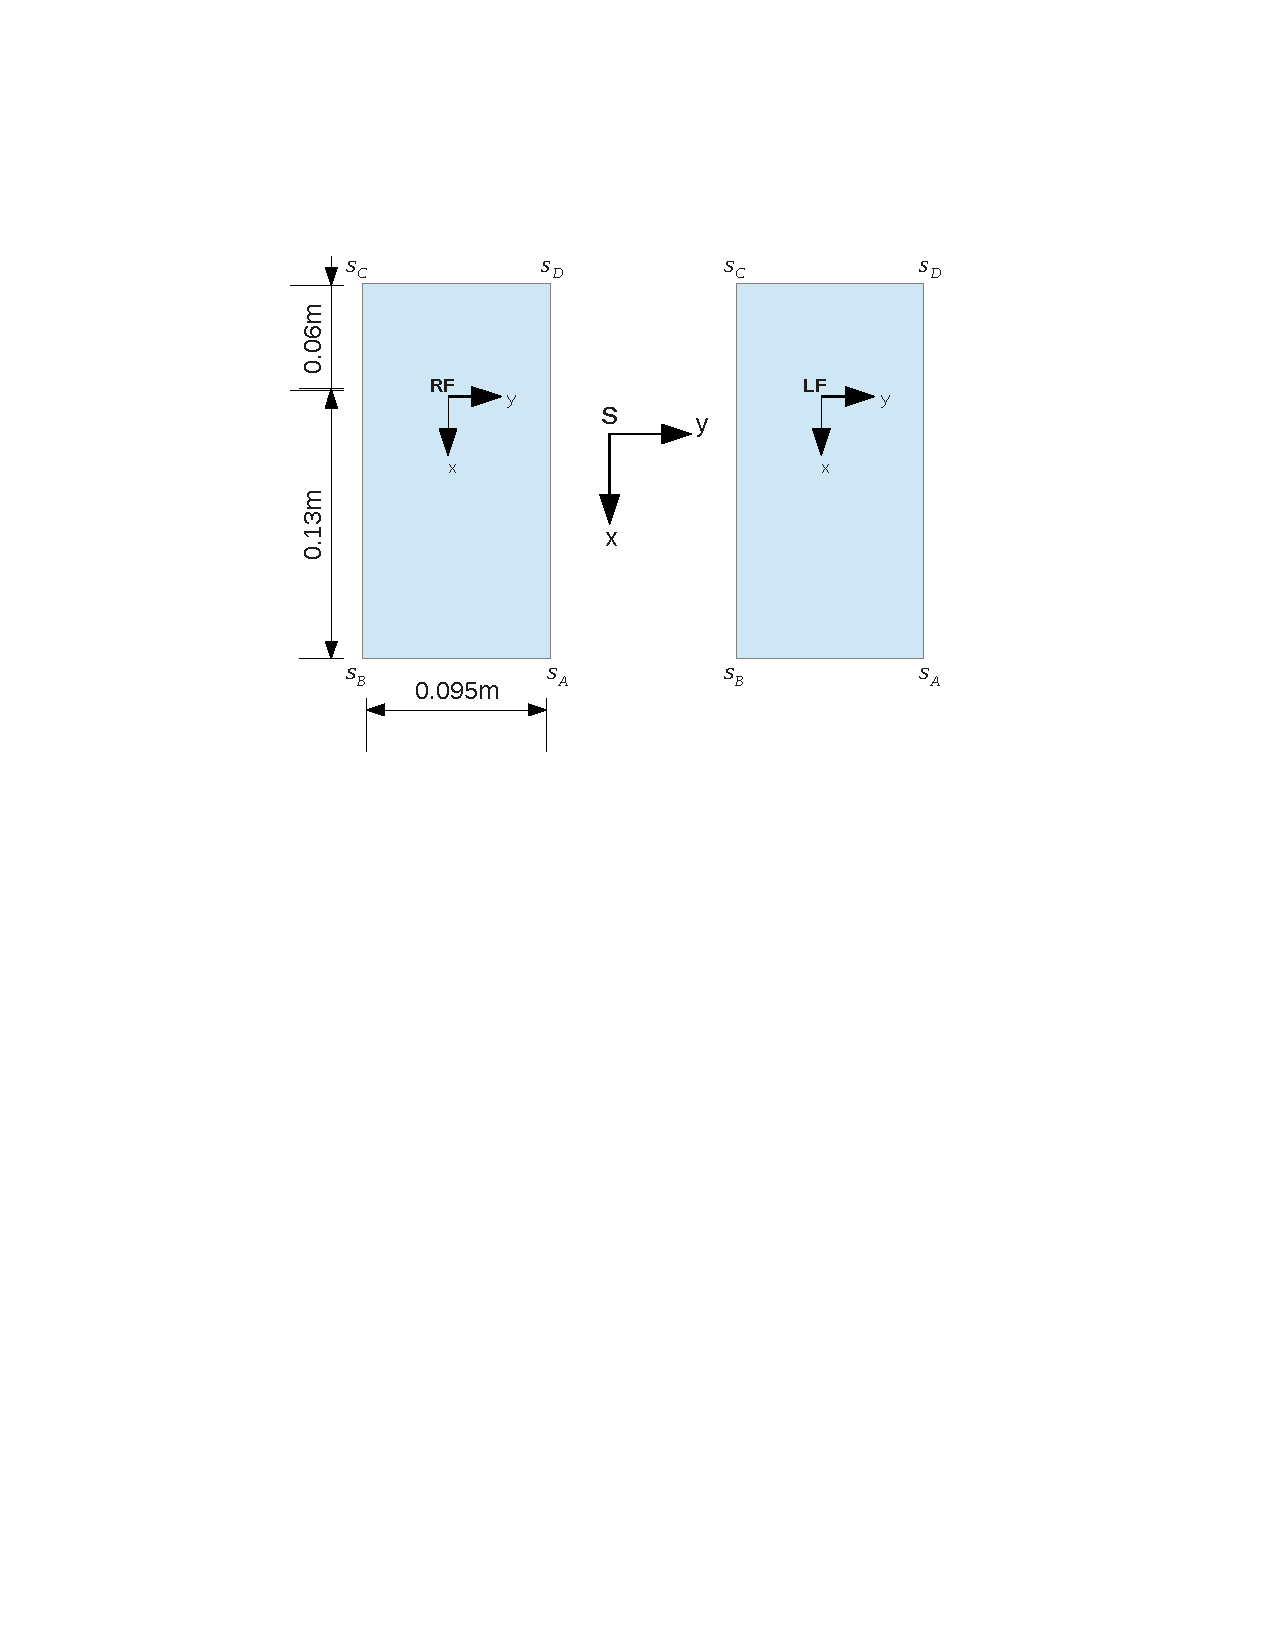
\includegraphics[trim= 20mm 150mm 20mm 50mm,scale=0.80]{Bilder/foot_topview.pdf}
    \caption{Toro feet viewed from top}
    \label{fig:biped_feet}
    \end{center}
\end{figure}
Along with the sensor measurements kinematic constraints can also be introduced as measurements \citep{atk12}. The kinematic constraint that is considered as measurement is the position constraint. For instance when the robot is tilting around an edge, the position of the points that are lying on that edge does not change with respect to the spatial frame (world frame). 
 
 Figure \ref{fig:biped_feet} shows the contact points considered for measurements. The corner points of each foot are measured with respect to spatial frame \emph{S}. The measuremnt equation of these contact points are
\begin{equation}
    \label{eq:y_kin}
    y_{kin} = s_{contact} = \begin{bmatrix}s_{r}\\ s_{l}\end{bmatrix},
\end{equation} where
$s_{r},s_{l}$ are the vectors of contact points in right foot and left foot defined with respect to spatial frame. They are given as
\begin{equation}
	\label{eq:y_cnt}
    \begin{split}
    s_{r} &= \begin{bmatrix} s_{A,r}\\ s_{B,r}\\ s_{C,r}\\ s_{D,r}\end{bmatrix}= \begin{bmatrix} {H}_{r}s_{A}\\  {H}_{r}s_{B}\\  {H}_{r}s_{C}\\  {H}_{r}s_{D}\end{bmatrix} \\
    s_{l} &= \begin{bmatrix} s_{A,l}\\ s_{B,l}\\ s_{C,l}\\ s_{D,l}\end{bmatrix}= \begin{bmatrix} {H}_{l}s_{A}\\  {H}_{l}s_{B}\\  {H}_{l}s_{C}\\  {H}_{l}s_{D}\end{bmatrix} \\
    \end{split}
\end{equation}
where ${H}_{r},{H}_{l}$ are the homogeneous transformation matrices of the right and left foot with respect to spatial frame [Appendix \ref{sec:htm}]
 In Figure \ref{fig:biped_feet} $s_A,s_B,s_C,s_D$ are constant with resptect to the foot coordinate frames \emph{RF,LF}. They are given as 
 $$ s_A = \begin{bmatrix} 0.13 \\ 0.0475 \\ 0 \end{bmatrix} , 
    s_B = \begin{bmatrix} 0.13 \\ -0.0475 \\ 0 \end{bmatrix},
    s_C = \begin{bmatrix} -0.06 \\ -0.0475 \\ 0 \end{bmatrix} \text{ and }
    s_D = \begin{bmatrix} -0.06 \\ 0.0475 \\ 0 \end{bmatrix}.$$

\paragraph{Contact switching:} The measurement of the contact points $s_{cnt}$\footnote{$s_{cnt}$ is the short form of $s_{contact}$ in Equation \ref{eq:y_kin}.} with respect to the spatial frame (world coordinate frame) are made before starting the experiment. These measurements are made under the circumstance where the feet of the robot make surface contact with the ground. For instance when the robot is standing on one foot then the contact measurements from the other foot are not valid. A parameter $\alpha$, that makes use of the vertical reaction force $F_z$ measured by Force Torque Sensor (FTS) on each foot to determine the support case \citep{atk12}:$$ \alpha = \frac{F_{z,r} + F_{z,l}}{F_{z,r}}.$$ 

\begin{figure}[H]
	% Define a few styles and constants
\tikzstyle{smallbox}=[draw, top color=white, bottom color=blue!20, text width=5em,text centered, minimum height=2.5em]
\tikzstyle{relationship} = [diamond,top color=white,bottom color=red!20,draw=red!50!black!100]

\centering
\begin{tikzpicture}[node distance=2cm]
	% Define the nodes in the picture
	\node (fts) {FTS};
	\node (contact_detect) [relationship,below of=fts]{Case $\alpha$};
	\node (LF) [smallbox,below of=contact_detect]{Left foot support};
	\node (RF) [smallbox,left of=LF,node distance= 3cm]{Right foot support};
	\node (DS) [smallbox,right of=LF,node distance= 3cm]{Double support};
	
	% Define edges
	\draw [->] (fts) --node{}(contact_detect);
	\draw [->] (contact_detect.west) -|node[above]{$\alpha\approx1$}(RF.north);
	\draw [->] (contact_detect.south) --node[left]{$\alpha\approx0$}(LF.north);
	\draw [->] (contact_detect.east) -|node[above]{$\alpha\approx0.5$}(DS.north);
	
\end{tikzpicture}
	\caption{Foot support cases determined using parameter $\alpha$}
	\label{fig:support_cases}
\end{figure}

The valid contact points are chosen based on the support case in Figure \ref{fig:support_cases}. The validity of the contact measurements can also change based on the type of contact the robot makes with the ground. For instance let us consider the robot is standing on its right leg. When the robot is tilting about the back edge of the foot, the front edge lifts off the ground which implies the contact changes from surface to line. The robot is only supported by the back edge of the foot. In this case the measurements of points $s_{C,r}$ and $s_{D,r}$ are valid, but $s_{A,r}$ and $s_B,r$ are invalid. So it is important to determine the state of contact of the robot with ground (surface or line). 

The Zero moment point (ZMP) is an useful criteria for detecting the state of contact. The coordinates of ZMP = $[{zmp}_{x},{zmp}_{y}]^T$ are defined with respect to the foot coordinate frame. As long as the ZMP is inside the support polygon\footnote{The support polygon refers to the surface of the foot that is in contact with the ground.} the robot will be in surface contact. The ZMP cannot be outside the support polygon (foot) \citep{mio04}. When the ZMP is located at the boundary of the support polygon then the robot changes from surface to line contact. In this case the contact will be about the line where the ZMP is located. Figure \ref{fig:biped_feet} shows the support polygons of right and left foot of \emph{Toro}. For instance when the ZMP is located at the back edge of a right foot's support in Figure \ref{fig:biped_feet}, then the contact is about the line (CD\footnote{From here on the line joining the points $s_X$ and $s_Y$ will be represented by XY.}) joining points $s_C$ and $s_D$. In this case the robot starts tilting about the line CD.
 
\begin{figure}[H]
	% Define a few styles and constants
\tikzstyle{smallbox}=[draw, top color=white, bottom color=blue!20, text width=5em,text centered, minimum height=2.5em]
\tikzstyle{relationship} = [diamond,top color=white,bottom color=red!20,draw=red!50!black!100]
\tikzstyle{bigbox} = [sensor,text width=6em,fill=green!30,minimum height=5em,rounded corners]
\tikzstyle{input} = [coordinate]
\tikzstyle{sum} = [draw, fill=blue!20, circle, node distance=1cm]
%\tikzstyle{output} = [coordinate]
\def\blockdist{0.5}
\def\edgedist{0.7}

\begin{tikzpicture}[node distance=2.5cm, scale=0.9]
	\node (FTS) {FTS};
	\node (ZMP)[smallbox,below of=FTS]{Compute ZMP};
	\node (RF_ZMPX) [relationship,below of=ZMP,xshift=3.5cm]{${\text{zmp}}_x$};
	\node (RF_TBACK) [smallbox,below of=RF_ZMPX,xshift=2cm]{Contact along line AB};
	\node (RF_TFRONT) [smallbox,left of=RF_TBACK,node distance=4cm]{Contact along line BC};	
	\node (RF_ZMPY) [relationship,left of=RF_ZMPX,node distance=7cm]{${\text{zmp}}_y$};
	\node (RF_TIN) [smallbox,below of=RF_ZMPY,xshift=2cm]{Contact along line BC};
	\node (RF_TOUT) [smallbox,left of=RF_TIN,node distance=4cm]{Contact along line AD};
	
	\draw [->] (FTS) --node{} (ZMP.north);
	\draw [->] (ZMP.east) -|node[right,text width=5em]{ZMP at vertical boundaries}(RF_ZMPX.north);
	\draw [->] (RF_ZMPX.east) -|node[above]{$< -0.05$}(RF_TBACK.north);
	\draw [->] (RF_ZMPX.west) -|node[above]{$> 0.12$}(RF_TFRONT.north);
	\draw [->] (ZMP.west) -|node[left,text width=5em]{ZMP at horizontal boundaries}(RF_ZMPY.north);
	\draw [->] (RF_ZMPY.east) -|node[above]{$< -0.04$}(RF_TIN.north);
	\draw [->] (RF_ZMPY.west) -|node[above]{$> 0.04$}(RF_TOUT.north);
	
	\begin{pgfonlayer}{background}
        % Compute a few helper coordinates
        \path (RF_TOUT.west |- ZMP.north)+(-0.8,0.8) node (a) {};
        \path (RF_TOUT.south -| RF_TBACK.east)+(0.8,-0.8)  node (b) {};
        \path[fill=yellow!20,rounded corners, draw=black!50, dashed]
            (a) rectangle (b);
     \end{pgfonlayer}
\end{tikzpicture}
 
	\caption{Line contacts of left foot in Figure \ref{fig:biped_feet} determined by \emph{ZMP}}
	\label{fig:zmp_cases}
\end{figure}

Each tilting case in Figure \ref{fig:zmp_cases} have different sets of contact points. The Algorithm \ref{alg:cnt_switch} is useful in making the decision about the contact points $s_{cnt}$ based on number of support and state of contact.
\begin{algorithm}
    \caption{Selection of contact measurements}
    \label{alg:cnt_switch}
    \begin{algorithmic}
    %\REQUIRE  $s_{cnt}$
    %\ENSURE $FOO$
    \IF {$\alpha = 0.5$}
    \STATE {Double support}
        \IF {$ {zmp}_x \geq 0.12$}
        \STATE Contact along line AB
        \RETURN $ s_{cnt}= \begin{bmatrix}s_{A,r} &s_{B,r} &s_{A,l} &s_{B,l} \end{bmatrix}^T$ 
        \ELSIF {${zmp}_x \leq -0.05$}
        \STATE Contact along line CD
        \RETURN $ s_{cnt}= \begin{bmatrix}s_{C,r} &s_{D,r} &s_{C,l} &s_{D,l} \end{bmatrix}^T$ 
        \ENDIF
    \ELSIF {$\alpha = 1$}
    \STATE Right foot support
        \IF {$ {zmp}_x \geq 0.12$}
        \STATE {Contact along line AB}
        \RETURN $ s_{cnt}= \begin{bmatrix}s_{A,r} &s_{B,r}  \end{bmatrix}^T$ 
        \ELSIF {${zmp}_x \leq -0.05$}
        \STATE Contact along line CD
        \RETURN $ s_{cnt}= \begin{bmatrix}s_{C,r} &s_{D,r}  \end{bmatrix}^T$ 
        \ELSIF {$ {zmp}_y \geq 0.04$}
        \STATE Contact along line AD
        \RETURN $ s_{cnt}= \begin{bmatrix}s_{A,r} &s_{D,r}  \end{bmatrix}^T$ 
        \ELSIF {${zmp}_y \leq -0.04$}
        \STATE Contact along line BC
        \RETURN $ s_{cnt}= \begin{bmatrix}s_{B,r} &s_{C,r}  \end{bmatrix}^T$ 
        \ENDIF
    \ELSIF {$\alpha = 0$}
    \STATE Support left foot
        \IF {$ {zmp}_x \geq 0.12$}
        \STATE Contact along line AB
        \RETURN $ s_{cnt}= \begin{bmatrix} s_{A,l} &s_{B,l} \end{bmatrix}^T$ 
        \ELSIF {${zmp}_x \leq -0.05$}
        \STATE Contact along line CD
        \RETURN $ s_{cnt}= \begin{bmatrix} s_{C,l} &s_{D,l} \end{bmatrix}^T$ 
        \ELSIF {$ {zmp}_y \geq 0.04$}
        \STATE Contact along line AD 
        \RETURN $ s_{cnt}= \begin{bmatrix}s_{A,r} &s_{D,r}  \end{bmatrix}^T$ 
        \ELSIF {${zmp}_y \leq -0.04$}
        \STATE Contact along line BC 
        \RETURN $ s_{cnt}= \begin{bmatrix}s_{B,r} &s_{C,r}  \end{bmatrix}^T$ 
        \ENDIF
    \ENDIF
    \end{algorithmic}
\end{algorithm}


The full measurement equations of the system is obtained by combining Equations \ref{eq:y_sens} and \ref{eq:y_kin}. The discretized form of measurement equations is
\begin{equation}
    \label{eq:y_msr}
    y_{k+1} = \begin{bmatrix} y_{sens,k+1} \\ y_{kin,k+1} \end{bmatrix}= \begin{bmatrix} acc^b_{k+1} \\ \omega^b_{k+1} \\ q_{k+1} \\ \dot q_{k+1} \\ s_{cnt,k+1} \end{bmatrix}.
\end{equation}

%\section{Prediction step}
\subsection{Prediction step}
\label{subsec:toro_predict}
The prediction equations of EKF given in Equation \ref{eq:ekf_predict} are as follows:
\begin{equation}
\label{eq:predict}
\begin{split}
\hat{x}_{k+1}^- &= f(\hat{x}_{k},u_{k+1},0)\\
P_{k+1}^- &= A_kP_{k}A_k^T + W_kQ_{k}W_k^T \\
\end{split}
\end{equation}
The state space model of \emph{Toro} in \ref{eq:toro} is discretized for the implementation of EKF. For smaller integration time steps $\Delta t = 1ms$ the forward Euler discretization method can be used to discretize the continuous time model. The forward Euler discretization equation is $$ x_{k+1} = x_k + \Delta t f(x),$$ where $f(x)=\dot x$ is the nonlinear function describing the system. The discretized prediction equation of \emph{Toro} is obtained by substituting $0$ for noise terms $w_\tau, w_{W_r}$ and $w_{W_l}$ in Equation \ref{eq:toro} and applying the forward Euler discretization:
\begin{equation}
\label{eq:toro_dis}
	\begin{bmatrix}
	\hat{p}_{k+1}^- \\ \hat{\theta}_{k+1}^- \\ \hat{q}_{k+1}^- \\ \hat{\dot{y}}_{k+1}^-
	\end{bmatrix}
	 =   
	 \begin{bmatrix}
	 \hat{p}_k \\ \hat{\theta}_k \\ \hat{q}_k \\ \hat{\dot{y}}_{k}
	\end{bmatrix}	  
	+ \Delta t f(\hat{x}_k,u_{k+1}) \\
\end{equation}
$$ f(\hat{x}_k,u_{k+1})\footnotemark[1] = 
	\begin{bmatrix}
	\hat R_k \hat v^b_k \\
	\hat T_k^{-1} \hat \omega_k^b  \\
	\hat{\dot{q}}_k\\
	M(\hat{y}_{k})^{-1}(-C(\hat{y}_{k},\hat{\dot{y}}_{k})\hat{\dot{y}}_{k} -g(\hat{y}_{k}) +  J_r(\hat{y}_{k})^{T}W_{r,k+1} +J_l(\hat{y}_{k})^{T}W_{l,k+1} + \tau_{k+1})	
	\end{bmatrix}  $$
where $\hat{x}(t_k) = \hat{x}(k \Delta t) = \hat{x}_k$ represents the state x at \emph{kth} sampling instant. $\hat{x}_{k+1} = \hat{x}(k \Delta t + \Delta t)$ represents the state of the system at the next sampling instant. $u_{k+1}$ is the input at sampling instant $k+1$. The inputs $\tau, W_l, W_r$ remains constant in the interval between two sampling instant because of the zero order hold mechanism in the sensor. The above equation is used to predict the state $\hat{x}_k$ ahead of time in Equation \ref{eq:predict}. 
\footnotetext[1]{$\hat R_k, \hat T_k$ are the shorthand notations for $R(\hat \theta_k)$ and $T(\hat \theta_k)$ in the equation.}

For the computation of state covariance matrix $P_k^-$ in Equation \ref{eq:predict}, the Jacobian matrix $A$ should be computed. The Jacobian matrix is the matrix of first order partial derivatives of a vector valued function \citep{wal76}.

The Jacobian matrix computation of the prediction Equations \ref{eq:toro_dis} of EKF is as follows:
\begin{enumerate}
\item The prediction equation for the position of the base is $ \hat{p}_{k+1}^- = \hat{p}_k + \Delta t \hat R_k \hat v^b_k$, where  $ \hat{p}_k = [\hat{p}_{x,k},\hat{p}_{y,k},\hat{p}_{z,k}]$ is the coordinates of position at time instant $k$. The Jacobian matrix of the equation is given by
\begin{equation}
\label{eq:dpdx}
\dfdx{\hat{p}_{j,k+1}^-}{x} = \left(\dfdx{\hat{p}_{j,k+1}^-}{x_{1}}, \dfdx{\hat{p}_{j,k+1}^-}{x_{2}}, \cdots , \dfdx{\hat{p}_{j,k+1}^-}{x_{62}}\right) \in \Re^{3 \times 62} \hspace{2cm} j=1,2,3
\end{equation}
\[
 \dfdx{\hat{p}_{k+1}^-}{x_{i}} =  \left\lbrace
  \!\begin{aligned}
   &e_i & \text{if }(i=j)\\
   &\Delta t \dfdx{\hat R_k}{x_i} \hat v^b_k & \text{if }(3 < i \leq 6)\\
   &\textbf{0}_{3 \times 1} &\text{if }(6 < i \leq 31) \text{ or } (35 < i \leq 62) \\
   &col(\hat R_k,i-31) & \text{if } 31 < i \leq 34 \\
  \end{aligned} \right.
\]where
\begin{itemize}
\item the subscript \emph{j} represents the row dimension and \emph{i} represents the column dimension of the Jacobian matrix,
\item $col(X,i)$ - represents the $i^{th}$ column of matrix $X$,
\item the partial derivative of \emph{R} with respect to the state $\hat{x}_k$ is $\dfdx{\hat R_k}{x_i}$ [Appendix \ref{sec:rot_mat}]),
\item  $e_i$ is the unit vectors in direction of coordinate axis and  $\textbf{0}_{3 \times 1}$ is the zero vector of dimensions 3 [Appendix \ref{sec:symbols}].
\end{itemize}

\item The prediction equation for the orientation of the base is $\hat{\theta}_{k+1}^- = \hat{\theta}_k + \Delta t \hat T_k^{-1} \omega_k^b$, where $\hat \theta_k = [ \theta_{x,k},\theta_{y,k},\theta_{z,k}]$ are the coordinates of orientation of the base. The Jacobian matrix of the equation is given by
\begin{equation}
\label{eq:dthetadx}
\dfdx{\hat{\theta}_{j,k+1}^-}{x} = \left(\dfdx{\hat{\theta}_{j,k+1}^-}{x_{1}}, \dfdx{\hat{\theta}_{j,k+1}^-}{x_{2}}, \cdots , \dfdx{\hat{\theta}_{j,k+1}^-}{x_{62}}\right) \in \Re^{3 \times 62}
\end{equation}
\[
 \dfdx{\hat{\theta}_{k+1}^-}{x_{i}} = \left\lbrace
  \!\begin{aligned}
   &\textbf{0}_{3 \times 1} &\text{if }(0 < i \leq 3) \text{ or }(6 < i \leq 31) \\
   &\hspace{2cm} &\text{ or } (35 < i \leq 62) \\
   &e_{i-3} + \Delta t \dfdx{\hat T_k^{-1}}{x_i}\omega_k^b & \text{if}3< \text{i} \leq 6 \\
   &col(\hat T_k^{-1},i-34) & \text{if } 31 < i \leq 34 \\
  \end{aligned} \right.
\]where
\begin{itemize}
\item $\dfdx{\hat T_k^-}{x_i}$ is the partial derivative of inverse of transformation matrix with respect to state [Appendix \ref{sec:avel_trfm}].
\end{itemize}

\item The prediction equation for the joint angles of multibody system is  $\hat{q}_{k+1}^- = \hat{q}_k + \Delta t \hat {\dot{q}}_k $. The Jacobian matrix of the equation is given by
\begin{equation}
\label{eq:dqdx}
\dfdx{\hat{q}_{k+1}^-}{x} = \left(\dfdx{\hat{q}_{k+1}^-}{x_{1}}, \dfdx{\hat{q}_{k+1}^-}{x_{2}}, \cdots , \dfdx{\hat{q}_{k+1}^-}{x_{62}}\right) \in \Re^{25 \times 62}
\end{equation}
\[
\dfdx{\hat{q}_{k+1}^-}{x_{i}} = 
	\begin{cases}
	l_{25,i} & \text{if } (6 < i \leq 31) \text{ or } (38 < i \leq 62) \\
	0 & \text{otherwise}   \\
	\end{cases}
\]where
\begin{itemize}
\item $l_{25,i}$ is a column vector of length 25 with 1 in the $i^{th}$ position and zeros in other position [Appendix \ref{sec:symbols}].
\end{itemize}

\item The prediction equation for the velocities of the robot is $\hat{\dot{y}}_{k+1}^- = \hat{\dot{y}}_{k}+ \Delta t \Lambda $, where 
$$\Lambda = M(\hat{y}_{k})^{-1}(-C(\hat{y}_{k},\hat{\dot{y}}_{k})\hat{\dot{y}}_{k} - g(\hat{y}_{k}) + J_r(\hat{y}_{k})^{T}W_{r,k+1} +J_l(\hat{y}_{k})^{T}W_{l,k+1} + \tau_{k+1})$$
The Jacobian matrix of the equation is given by
 \begin{equation}
 \label{eq:dydx}
\dfdx{\hat{\dot{y}}_{k+1}^-}{x} = \left(\dfdx{\hat{\dot{y}}_{k+1}^-}{x_{1}}, \dfdx{\hat{\dot{y}}_{k+1}^-}{x_{2}}, \cdots , \dfdx{\hat{\dot{y}}_{k+1}^-}{x_{62}}\right) \in \Re^{31 \times 62}
\end{equation}
where
\[
\dfdx{\hat{\dot{y}}_{k+1}^-}{x_{i}} = 
\left\{ 
\!\begin{aligned}
	& \left. \!\begin{aligned}
	-M_k^{-1}\dfdx{M_k}{x_{i}}\Lambda + &M_k^{-1}\left(-\dfdx{C_k}{x_{i}}\hat{\dot{y}}_{k} -\dfdx{g_k}{x_{i}}+ \right. \\
	&\left(\dfdx{J_{r,k}}{x_{i}}\right)^{T}W_{r,k+1} + \left. \left(\dfdx{J_{l,k}}{x_{i}}\right)^{T}W_{l,k+1} \right)
	\end{aligned} \right\}& \text{if } 0 < i \leq 31 \\
    & \left.\!\begin{aligned}
    l_{31,(i-31)}-&M_k^{-1}\dfdx{M_k}{x_{i}}\Lambda+ \\
    &M_k^{-1}\left(-\dfdx{C_k}{x_{i}}\hat{\dot{y}}_{k}- col(C_k,i-31)\right)     
    \end{aligned} \right\} & \text{if } i < 31  \\
\end{aligned}
\right.
\]where
\begin{itemize}
\item the shorthand form symbols used are  $M_k= M(\hat{y}_{k}),C_k=C(\hat{y}_{k},\hat{\dot{y}}_k),J_{r,k}=J_r(\hat{y}_{k}),J_{l,k}=J_l(\hat{y}_{k})$
\end{itemize}
\end{enumerate}
The system matrix $A_k$ is formulated by combining Equations \ref{eq:dpdx},\ref{eq:dthetadx},\ref{eq:dqdx} and \ref{eq:dydx} as
\begin{equation}
\label{eq:sys_mat}
A_k = \left(
\begin{aligned}
\dfdx{\hat{p}_{k+1}^-}{x} \\
\dfdx{\hat{\theta}_{k+1}^-}{x} \\
\dfdx{\hat{q}_{k+1}^-}{x}\\
\dfdx{\hat{\dot{y}}_{k+1}^-}{x}
\end{aligned} \right)
\in \Re^{62 \times 62}
\end{equation}

The noise correlation matrix $W_k$ is derived by discretizing the Equation \ref{eq:toro} and computing the Jacobian matrix of the discretized equation with respect to the noise $w$. Discretization of the Equation \ref{eq:toro} will result in a equation similar to \ref{eq:toro_disc}. The matrix $W_k$ is 
\begin{equation}
    \label{eq:toro_noisecorr}
    W_k =  \begin{bmatrix}
        \textbf{0}_{31,31} \\ 
        J_{r,k}^T \hspace{5mm} J_{l,k}^T \hspace{5mm} col(7:31,M_k^{-1})
        \end{bmatrix},
\end{equation}
where $\textbf{0}_{31,31}$ is a zero matrix of dimension $31 \times 31$, $col(7:31,M_k^{-1})$ represents the $7^{th}$ to ${31}^{st}$ colomns of the $M_k^{-1}$ matrix.

Substituting Equations \ref{eq:toro_dis}, \ref{eq:sys_mat} and \ref{eq:toro_noisecorr} in \ref{eq:predict} and substituting the values of process covariance $Q_k$ completes the prediction stage of EKF.


%\section{Update step}
\subsection{Update step}
\label{subsec:toro_update}
The update equation of the EKF is given in Equation \ref{eq:ekf_correct}. The measurement equation of the system is given by $$\hat{y}_{k+1} = h(\hat{x}_{k+1}^-,u_{k+1},0).$$ For the sake of simplicity let us assume the measurement of noise uncorrelated. That is the noise acting on a measurement does not depend on the noise acting on all other measurements. $$V_k = I_3.$$ Substituting the assumption in Equation \ref{eq:ekf_correct} gives
\begin{equation}
\label{eq:correct}
\begin{split}
K_{k+1} &= P_{k+1}^-\hat{C}_{k+1}^{T-}(\hat{C}_{k+1}^-P_{k+1}^-\hat{C}_{k+1}^{T-} + R_{k+1})^{-1}\\
\hat{x}_{k+1} &= \hat{x}_{k+1}^- + K_{k+1}(y_{k+1}-\hat{y}_{k+1})\\
P_{k+1} &= (I- K_{k+1}\hat{C}_{k+1}^-)P_{k+1}^-.
\end{split}
\end{equation}
The measurements of \emph{Toro} are Cartesian accelerations($acc^b$) of the hip measured by accelerometer, angular velocity($\omega^b$) of the hip measured by the gyroscope, joint angles($q_j$) and joint velocities($\dot{q_j}$) measured by joint encoders.
\begin{equation}
    \label{eq:y_sens}
     y_{sens} = \begin{bmatrix} acc^b \\ \omega^b \\ q_j \\ \dot{q}_j \end{bmatrix} 
\end{equation}
\begin{itemize}
    \item The simplified model of $IMU_{acc}$ is $$ acc^b= \begin{bmatrix} acc^b_x \\ acc^b_y \\ acc^b_z \end{bmatrix} =  \begin{bmatrix}\ddot{p}_x^b \\ \ddot{p}_y^b \\ \ddot{p}_z^b \end{bmatrix} - R^T \begin{bmatrix}0 \\0 \\-9.81 \end{bmatrix}$$ \emph{R} is the rotational matrix that transforms a vector in body coordinate frame to spatial frame.
    \item $\ddot{p}^b$ is computed from the forward dynamic equation \ref{eq:motion} using the predicted values of the state
    \item $\omega_{f}^{b} $ is the vector of angular rates of the hip(floating base) measured by gyroscope. The measurements are in the frame attached to the hip. 
\end{itemize}
\begin{figure}
    \begin{center}
    %trim option's parameter order: left bottom right top
    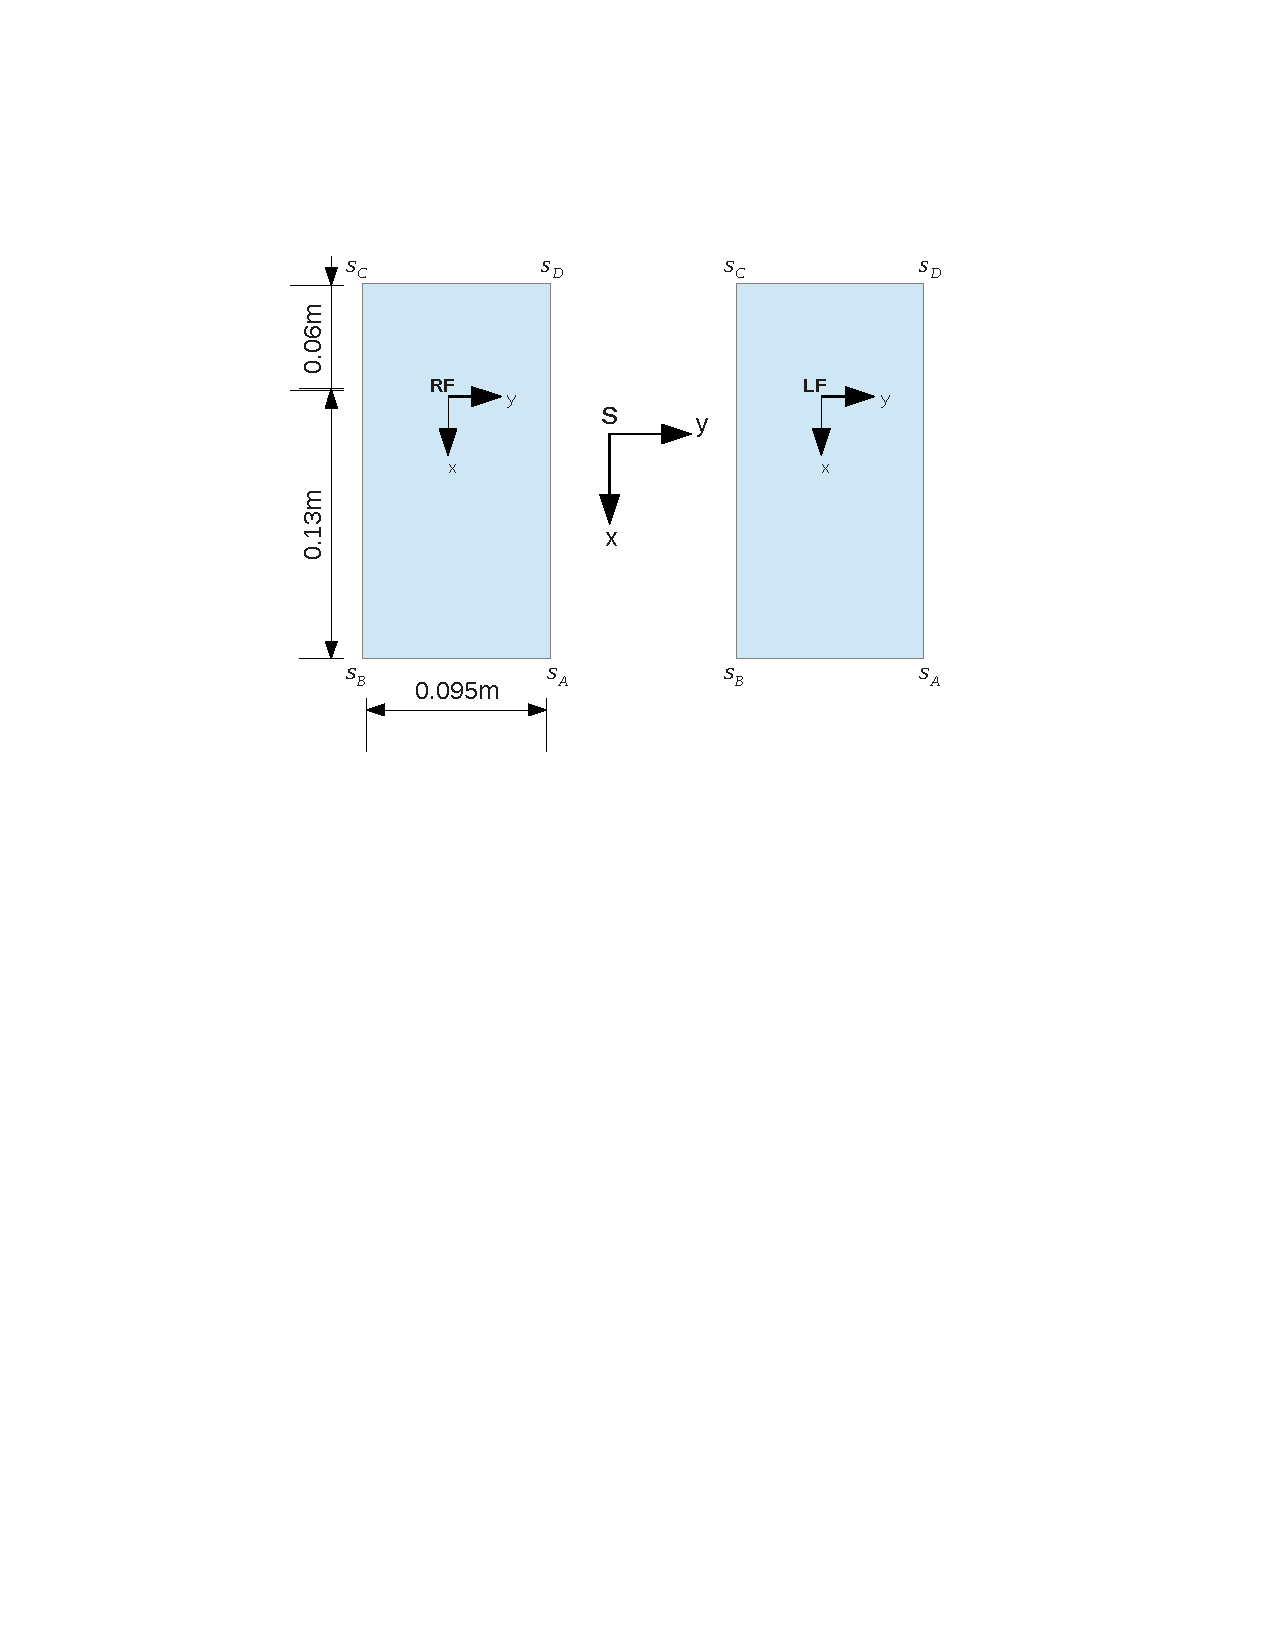
\includegraphics[trim= 20mm 150mm 20mm 50mm,scale=0.80]{Bilder/foot_topview.pdf}
    \caption{Toro feet viewed from top}
    \label{fig:biped_feet}
    \end{center}
\end{figure}
Along with the sensor measurements kinematic constraints can also be introduced as measurements \citep{atk12}. The two kinematic constraints considered as measurement are velocity constraints and position constraints. For instance when a foot is in contact with the ground the velocity of the foot is zero. The velocity of a end-effector $V^{eff}$ is \citep[chapter 3]{mur94} 
\begin{equation}
    V^{eff} = J(q) \dot q
\end{equation}
where $J(q)$ is the body Jacobian that maps the joint angular velocities $\dot q$ to the end effector velocity $V^{eff}$. In addition to the velocity constraints we can introduce position constraints. For instance when the robot is tilting around an edge, the position of the points that are lying on the edge does not change with respect to the world. 
 Figure \ref{fig:biped_feet} shows the contact points considered for measurements. The corner points of each foot are measured with respect to spatial frame \emph{S} as shown in Figure \ref{fig:biped_feet} before starting the experiment and they are assumed to be constant throughout the experiment.
\begin{equation}
    \label{eq:y_kin}
    \begin{split}
    y_{kin} &=
    \begin{bmatrix}
    p_{contact} \\ V_{contact}
    \end{bmatrix}\\
    p_{contact} &= \begin{bmatrix}p_{r}\\ p_{l}\end{bmatrix}\\
     V_{contact} &= \begin{bmatrix} V_{r}^b \\ V_{l}^b \end{bmatrix} = \begin{bmatrix} J_r(\hat{y})^T \hat{\dot{y}} \\ J_l(\hat{y})^T\hat{\dot{y}} \end{bmatrix}
    \end{split}
\end{equation}
\begin{itemize}
\item $p_{r},p_{l}$ are the vectors of contact points in right foot and left foot defined with respect to spatial frame.
\item $J_r(y), J_l(y)$ are the body Jacobian of right and left foot that relates the joint velocity to the velocity of right and left foot respectively.
\end{itemize}
\begin{equation}
    \begin{split}
    p_{r} &= \begin{bmatrix} p_{A,r}\\ p_{B,r}\\ p_{C,r}\\ p_{D,r}\end{bmatrix}= \begin{bmatrix} {H}_{r}p_{A}\\  {H}_{r}p_{B}\\  {H}_{r}p_{C}\\  {H}_{r}p_{D}\end{bmatrix} \\
    p_{l} &= \begin{bmatrix} p_{A,l}\\ p_{B,l}\\ p_{C,l}\\ p_{D,l}\end{bmatrix}= \begin{bmatrix} {H}_{l}p_{A}\\  {H}_{l}p_{B}\\  {H}_{l}p_{C}\\  {H}_{l}p_{D}\end{bmatrix} \\
    \end{split}
\end{equation}
\begin{itemize}
\item $\hat{H}_{r},\hat{H}_{l}$ are the homogeneous transformation matrices of the right and left foot [Appendix \ref{sec:htm}]
\item In Figure \ref{fig:biped_feet} $p_A,p_B,p_C,p_D$ are the corner points defined with respect to respective foot frame \emph{r,l}.
\end{itemize}
The full measurement equations of the system is obtained by combining Equations \ref{eq:y_sens} and \ref{eq:y_kin}. The discretized form of measurement equations is
\begin{equation}
    \label{eq:y_msr}
    y_{k+1} = \begin{bmatrix} y_{sens,k+1} \\ y_{kin,k+1} \end{bmatrix}= \begin{bmatrix} acc^b_{k+1} \\ \omega^b_{k+1} \\ q_{k+1} \\ \dot q_{k+1} \\ p_{r,k+1} \\ p_{l,k+1} \\ V^b_{r,k+1} \\ V^b_{l,k+1} \end{bmatrix}.
\end{equation}

For the computation of Kalman gain $K_k$ and update the error covariance matrix $P_k$ in Equation \ref{eq:correct}, the measurement sensitivity matrix $C_k$ have to be computed. The matrix $C_k$ determined by computing the Jacobian matrix of the measurement equation \ref{eq:y_msr}. The computation of $C_k$ matrix is as follows:
\begin{enumerate}
\item The measurement equation for acceleration measurements is  $$\hat{acc}^b_{k+1} = \dot{v}^{b-}_{k+1}-\hat{R}_{k+1}^{T-}\begin{bmatrix} 0 \\ 0 \\ -9,81 \end{bmatrix}$$.
The Jacobian matrix is 
\begin{equation}
    \label{eq:dacc_msrdx}
    \dfdx{\hat{acc}_{k+1}^{b-}}{x} = \dfdx{\hat{\dot{v}}_{k+1}^{b-}}{x} - \dfdx{\hat{R}^{T-}_{k+1}}{x}\begin{bmatrix} 0 \\ 0 \\ -9,81 \end{bmatrix}  \in \Re^{3 \times 62}
\end{equation}where
\begin{itemize}
    \item $\dfdx{\hat{\dot{v}}_{k+1}^b}{x}$ is Jacobian matrix obtained by evaluating Equation \ref{eq:dydx} with the values $\hat x_{k+1}^-, u_{k+1}$ and picking the rows corresponding to the linear acceleration. For instance in Equation \ref{eq:dydx} the first three rows of the Jacobian matrix corresponds to the linear acceleration.
    \item $\dfdx{\hat{R}^T_{k+1}}{x}$ is partial derivative of Rotation matrix [Appendix \ref{sec:rot_mat}].
\end{itemize}

\item The Jacobian matrix corresponding to the angular velocity $\hat{\omega}^{b-}_{k+1}$ is 
\begin{equation}
    \label{eq:dw_msrdx} 
    \dfdx{\hat{\omega}^{b-}_{k+1}}{x} = \left(\dfdx{\hat{\omega}^{b-}_{k+1}}{x_{1}}, \dfdx{\hat{\omega}^{b-}_{k+1}}{x_{2}}, \cdots , \dfdx{\hat{\omega}^{b-}_{k+1}}{x_{62}}\right) \in \Re^{3 \times 62}
\end{equation}
\[ \dfdx{\hat{\omega}^{b-}_{k+1}}{x} = 
    \begin{cases}
    l_{3,i-34} & \text{if } 34 < i \leq 37 \\
    \textbf{0}_{3,1} &\text{otherwise}.
    \end{cases}
 \]where 
 \begin{itemize}  
 \item $l_{x,y}$ is a zero vector of length $x$ with 1 at the $y^{th}$ position.
 \item $\textbf{0}_{m,n}$ is the zero matrix of dimensions $m$ and $n$.
 \end{itemize}

\item The Jacobian matrix corresponding to the joint angles $\hat{q}_{k+1}^-$ is
\begin{equation}
\label{eq:dq_msrdx}
\dfdx{\hat{q}_{k+1}^-}{x} = \left(\dfdx{\hat{q}_{k+1}^-}{x_{1}}, \dfdx{\hat{q}_{k+1}^-}{x_{2}}, \cdots , \dfdx{\hat{q}_{k+1}^-}{x_{62}}\right) \in \Re^{25 \times 62}
\end{equation}
 \[
 \dfdx{\hat{q}_{k+1}^-}{x_{i}} =
 \begin{cases}
 l_{25,i-6} & \text{if } 6 < i \leq 31 \\
 \textbf{0}_{25,1} & \text{otherwise}.
 \end{cases}
 \]

\item The Jacobian matrix corresponding to the angular velocity of joint angles  $\hat{\dot{q}}_{k+1}^-$ is 
\begin{equation}
 \label{eq:ddq_msrdx}
\dfdx{\hat{\dot{q}}_{k+1}^-}{x} = \left(\dfdx{\hat{\dot{q}}_{k+1}^-}{x_{1}}, \dfdx{\hat{\dot{q}}_{k+1}^-}{x_{2}}, \cdots , \dfdx{\hat{\dot{q}}_{k+1}^-}{x_{62}}\right) \in \Re^{25 \times 62}
\end{equation}
  \[
 \dfdx{\hat{\dot{q}}_{k+1}^-}{x_{i}} =
 \begin{cases}
 l_{25,i-37} & \text{if } 37 < i \leq 62 \\
 \textbf{0}_{25,1} & \text{otherwise}.
 \end{cases}
 \]

 \item The measurement equation for the contact points in right foot is $$\hat{p}_{r,k+1}^- = \hat{H}_{r,k+1}^- p = \begin{bmatrix} \hat{H}_{r,k+1}^- p_{A}\\ \hat{H}_{r,k+1}^- p_{B}\\ \hat{H}_{r,k+1}^- p_{C}\\ \hat{H}_{r,k+1}^- p_{D}\end{bmatrix}.$$
 The Jacobian matrix is 
\begin{equation}
    \label{eq:dpr_msrdx}
    \begin{split}
    &\dfdx{\hat{p}_{r,k+1}^-}{x} = \dfdx{\hat{H}_{r,k+1}^-}{x}p\in \Re^{12 \times 62}
 \\ \vspace{1cm} \\
     \dfdx{\hat{H}_{r,k+1}^-}{x} = &\left( \dfdx{\hat{H}_{r,k+1}^-}{x_1}, \dfdx{\hat{H}_{r,k+1}^-}{x_2},\cdots, \dfdx{\hat{H}_{r,k+1}^-}{x_{62}} \right)     
     \end{split}
\end{equation}where
\begin{itemize}
     \item $\dfdx{\hat{H}_{r,k+1}^-}{x}$ is the derivative of homogeneous transformation matrix with respect to the system states [Appendix \ref{sec:htm}].
\end{itemize}
 \item The measurement equation for the contact points in left foot is  $\hat{p}_{l,k+1}^- = \hat{H}_{l,k+1}^- p$.

 The Jacobian matrix is 
\begin{equation}
    \label{eq:dpl_msrdx}
    \dfdx{\hat{p}_{l,k+1}^-}{x} = \dfdx{\hat{H}_{l,k+1}^-}{x}p\in \Re^{12 \times 62}
\end{equation}where
\begin{itemize}
    \item $\dfdx{\hat{p}_{l,k+1}^-}{x}$ is computed similar to $\dfdx{\hat{p}_{r,k+1}^-}{x}$ in Equation \ref{eq:dpr_msrdx}.
\end{itemize}

\item The measurement equation for the velocities of the right and left foot is  $$\hat{V}_{contact,k+1}^b = \begin{bmatrix} \hat{V}_{r,k+1}^{b-} \\ \hat{V}_{l,k+1}^{b-} \end{bmatrix} 
=\begin{bmatrix}\hat{J}_{r,k+1}^{T-} \hat{\dot{y}}_{k+1}\\ \hat{J}_{l,k+1}^{T-} \hat{\dot{y}}_{k+1}\end{bmatrix}$$
The Jacobian matrix is 
\begin{equation}
    \label{eq:dv_msrdx}
     \dfdx{\hat{V}_{cnt,k+1}^-}{x} = \left( \dfdx{\hat{V}_{cnt,k+1}^-}{x_1}, \dfdx{\hat{V}_{cnt,k+1}^-}{x_2},\cdots, \dfdx{\hat{V}_{cnt,k+1}^-}{x_{62}} \right)\in \Re^{12 \times 62}
\end{equation}
\[
\dfdx{\hat{V}_{cnt,k+1}^{-}}{x_{i}} = 
	\begin{cases}
	\left(
	\begin{aligned}
	\dfdx{\hat{J}_{r,k+1}^{T-}}{x_{i}}\dot{\hat{y}}^- \\
	\dfdx{\hat{J}_{l,k+1}^{T-}}{x_{i}}\dot{\hat{y}}^- \\
	\end{aligned} \right)
	& \text{if } 1 \leq i \leq 31 \\
	\begin{pmatrix}
	col(\hat{J}_{r,k+1}^{T-},i)\\ col(\hat{J}_{l,k+1}^{T-},i)
	\end{pmatrix}
	 	& \text{if } 32 \leq i \leq 62
	\end{cases}
\]where
\begin{itemize}
    \item $ \hat{V}_{cnt,k+1}^{-}$ is the shorthand notation for $\hat{V}_{contact,k+1}^{b-} $.
\end{itemize}
\end{enumerate}
The measurement sensitivity matrix $\hat{C}_{k+1}^-$ of the system is given by Equations \ref{eq:dacc_msrdx}, \ref{eq:dw_msrdx}, \ref{eq:dq_msrdx}, \ref{eq:ddq_msrdx}, \ref{eq:dpr_msrdx}, \ref{eq:dpl_msrdx} and \ref{eq:dv_msrdx}.
\begin{equation}
    \label{eq:msr_mat}
    \hat{C}^-_{k+1} = \left(
   \begin{aligned}
   \dfdx{\hat{acc}_{k+1}^{b-}}{x} \\
   \dfdx{\hat{\omega}^{b-}_{k+1}}{x} \\
    \dfdx{\hat{q}_{k+1}^-}{x} \\
    \dfdx{\hat{\dot{q}}_{k+1}^-}{x} \\
    \dfdx{\hat{p}_{r,k+1}^-}{x} \\
    \dfdx{\hat{p}_{l,k+1}^-}{x} \\
	 \dfdx{\hat{V}_{cnt,k+1}^{-}}{x} 
   \end{aligned}
	 \right) \in \Re^{80 \times 62}
\end{equation}

\begin{comment}
\paragraph{Observability:}
State space representation of a linear system is,
\begin{equation}
\label{eq:dyn_l}
\begin{split}
\dot{x} &= Ax + Bu\\
y &= Cx + Du.
\end{split}
\end{equation}
where, $x \in \Re^{n}$ is the vector representing the states of the system. $u \in \Re^{p}$ is the vector of inputs, $y \in \Re^{m}$ is the vector of outputs of the system. $A \in \Re^{n \times n}$ is the system matrix. $B \in \Re^{n \times p}$ is the matrix relating state and input, $C \in \Re^{m \times n}$ is the measurement matrix relating output and state, $D \in \Re^{m \times p}$ is the matrix relating input and output of the system.

Linearising a nonlinear system in Equation \ref{eqn:nl_sys} at some operating point will lead to linear system of form Eq. \ref{eq:dyn_l}. For a linear system to be observable, it should satisfy
\begin{equation}
obs =
\begin{pmatrix}
C\\ CA \\ CA^{2}\\ \vdots \\ CA^{n-1}
\end{pmatrix}
, rank(obs) =n
\end{equation}
For our system to be observable $rank(obs) = 62$.
\end{comment}
%\textbf{ Make plots from files act=datsrc/ROBOT-TILT-0807.mat est=estimates-data/est-090701.mat or *080703.mat }
%\end{document}


% Experiments 
\subsection{Experiment}
\label{subsec:toro_exp}
The estimation problem is tested in Matlab Simulink. The experimental setup consists of the Open HRP3 simulator and the state estimator. The OpenHRP3 (Open Architecture Human-centred Robotics Platform version 3) is an integrated software platform for robot simulations and software developments \footnote{\url{http://www.openrtp.jp/openhrp3/en/about.html}}. It was developed as a cooperative work of University of Tokyo, General Robotix. Inc and National Institute of Advanced Industrial Science and Technology(AIST).

\begin{figure}[H]
    \centering
    % We need layers to draw the block diagram
\pgfdeclarelayer{background}
\pgfdeclarelayer{foreground}
\pgfsetlayers{background,main,foreground}

% Define a few styles and constants
\tikzstyle{sensor}=[draw, fill=blue!20, text width=5em,text centered, minimum height=2.5em]
\tikzstyle{system} = [sensor, text width=6em, fill=green!30, 
    minimum height=12em, rounded corners]
\tikzstyle{input} = [coordinate]
\tikzstyle{sum} = [draw, fill=blue!20, circle, node distance=1cm]
%\tikzstyle{output} = [coordinate]
\def\blockdist{0.5}
\def\edgedist{0.75}
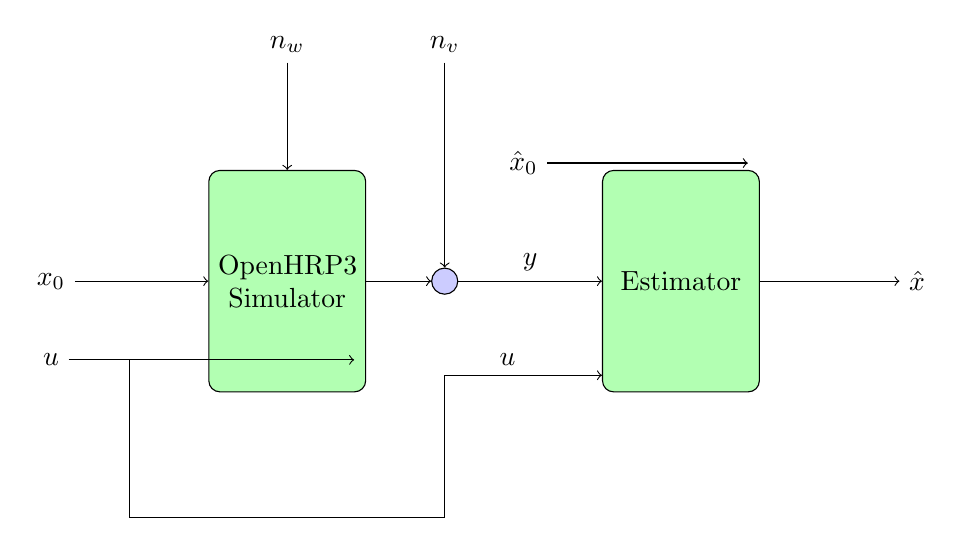
\begin{tikzpicture}
	% Define the nodes in the picture
	\node (sys_in)[yshift=1cm]{$x_0$};
	\node (u_in) [below of=sys_in,node distance=1cm]{$u$};
	\node (sys_u)[input,right of=u_in,node distance=1cm]{};
    \node (sim_sys) [system,right of=sys_in,node distance=3cm] {OpenHRP3 Simulator};
    \node (sys_noise)[above of=sim_sys,node distance=3cm]{$n_w$};
    \node (msr_noise)[right of=sys_noise,node distance=2cm]{$n_v$};
    \node (msr_add)[sum,right of=sim_sys,node distance=2cm]{};
    \node (estimator) [system,right of=msr_add,node distance =3cm]{ Estimator};
    \node (est_in) [right of=sim_sys,node distance=3cm,yshift=1.5cm]{$\hat{x}_0$};
    \node (est_u) [input,right of =sim_sys, node distance=2cm,yshift=-3cm]{foo};
    \node (est_out)[right of=estimator,node distance=3cm]{$\hat{x}$};
    
    % Define the edges in the picture
    \draw [->] (sys_in) --node{}(sim_sys.west);
    \draw [-] (u_in) --node{}(sys_u);
    \draw [->] (sys_u) --node{}+(\edgedist,0);
    \draw [-] (sys_u) |-node{}(est_u);
    \draw [->] (est_u) |-node[pos=0.7,above]{$u$}(estimator.-130);
    \draw [->] (est_in) --node{}+(\edgedist,0);
    \draw [->] (sys_noise) --node{}(sim_sys.north);
    \draw [->] (msr_noise) --node{}(msr_add.north);
    \draw [->] (sim_sys.east) --node[above]{}(msr_add.west);
    \draw [->] (msr_add.east) --node[above]{$y$}(estimator.west);
    \draw [->] (estimator) --node{}(est_out);
\end{tikzpicture}
    \caption{Experimental setup of TORO}
    \label{fig:toro_exp}
\end{figure}

A rigid body algorithm is used in the estimator to compute dynamic $M(y_k), C(y_k,\dot y_k), g(y_k)$ and kinematic $J_r(y_k), J_l(y_k), H(y_k)$ parameters at time step $k$. An auto differentiation function that computes the derivative of the dynamic and kinematic parameters with respect to the the system states is integrated with the rigid body algorithm. 
\begin{figure}[H]
    \centering
    % We need layers to draw the block diagram
\pgfdeclarelayer{background}
\pgfdeclarelayer{foreground}
\pgfsetlayers{background,main,foreground}

% Define a few styles and constants
\tikzstyle{sensor}=[draw, fill=blue!20, text width=5em,text centered, minimum height=2.5em, rounded corners]
\tikzstyle{system} = [sensor, text width=5em, fill=green!30, 
    minimum height=8em]
%\tikzstyle{input} = [coordinate]
\tikzstyle{sum} = [draw, fill=blue!20, circle, node distance=1cm]
\tikzstyle{output} = [coordinate]
%\def\blockdist{0.5}
\def\edgedist{2.85}
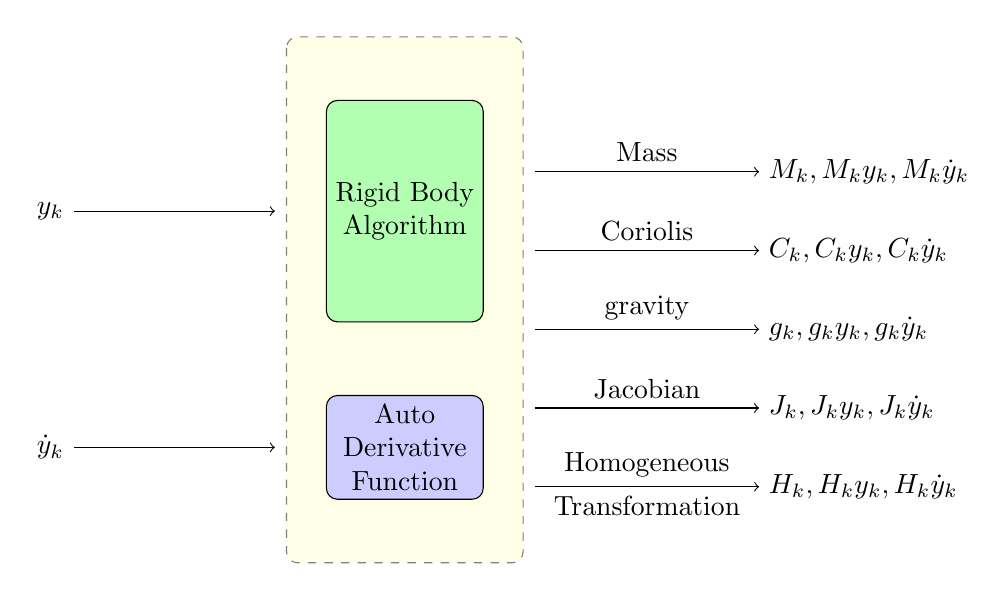
\begin{tikzpicture}
	% Define the nodes in the picture
	\node (y)[yshift=1cm]{$y_k$};
	\node (dy) [below of=y,node distance=3cm]{$\dot y_k$};
    \node (rigbdy_alg) [system,right of=y,node distance=4.5cm] {Rigid Body Algorithm};
    \node (auto_diff) [ sensor,below of=rigbdy_alg,node distance =3cm]{Auto Derivative Function};
    \node (M) [output,right of=rigbdy_alg,node distance=1.65cm,yshift=0.5cm]{};
    \node (C) [output,below of=M,node distance=1cm]{};
    \node (g) [output,below of=C,node distance=1cm]{};
    \node (J) [output,below of=g,node distance=1cm]{};
    \node (H) [output,below of=J,node distance=1cm]{};

    % Define the edges in the picture
    \draw [->] (y) --node{}+(\edgedist,0);
    \draw [->] (dy) --node{}+(\edgedist,0);
    \draw [->]  (M) --node[above]{Mass}+(\edgedist,0) node[right]{$M_k, \dfdx{M_k}{y_k},\dfdx{M_k}{\dot y_k}$};
    \draw [->]  (C) --node[above]{Coriolis}+(\edgedist,0) node[right]{$C_k, \dfdx{C_k}{y_k},\dfdx{C_k}{\dot y_k}$};
    \draw [->]  (g) --node[above]{gravity}+(\edgedist,0) node[right]{$g_k, \dfdx{g_k}{y_k},\dfdx{g_k}{\dot y_k}$};
    \draw [->]  (J) --node[above]{Jacobian}+(\edgedist,0) node[right]{$J_k, \dfdx{J_k}{y_k},\dfdx{J_k}{\dot y_k}$};
    \draw [->]  (H) --node[above]{Homogeneous} node[below]{Transformation}+(\edgedist,0) node[right]{$H_k, \dfdx{H_k}{y_k}, \dfdx{H_k}{\dot y_k}$};
    
    %Draw background layers
    \begin{pgfonlayer}{background}
        % Compute a few helper coordinates
        \path (auto_diff.west |- rigbdy_alg.north)+(-0.5,0.8) node (a) {};
        \path (auto_diff.south -| rigbdy_alg.east)+(+0.5,-0.8) node (b) {};
        \path[fill=yellow!10,rounded corners, draw=black!50, dashed]
            (a) rectangle (b);
    \end{pgfonlayer}
%\end{comment}
\end{tikzpicture}

    \caption{Structure of rigid body algorithm}
    \label{fig:luc_dyn}
\end{figure}
The Jacobian $J_k$ outputted by the algorithm shown in Figure \ref{fig:luc_dyn} is the body Jacobian of \emph{Toro's} right foot $J_r$ and left foot $J_l$ and homogeneous transformation matrix $H_k$ is the transformations of right foot $H_r$, left foot $H_l$ and floating base $H_b$ with respect to spatial frame (world frame).
The Jacobian matrices $A_k$ and $\hat C_{k+1}$ in Equations \ref{eq:sys_mat}, \ref{eq:msr_mat} are computed from these outputs of the rigid body algorithm. The formulation of the Jacobian matrices $A_k$ and $\hat C_{k+1}$ are discussed in sections \ref{subsec:toro_predict} and \ref{subsec:toro_update}. 

The simulator is driven by the control input $u$. For instance the control input of \emph{Toro} are the torque applied to joints $\tau$. The controller generates these inputs according to the control law. These inputs can be measured with the help of the torque sensors located at the joints. The ground reaction forces $W_r$ and $W_l$ are measured by the Force Torque sensor (FTS) located at the ankle joints. The ground reaction forces and the control torques are the input to prediction model in Equation \ref{eq:toro_dis}.

The following scenario is simulated using the OpenHRP3 simulator. It consists of the following phases:

\paragraph{Initial phase:} The robot is made to stand on the ground (high pose). After a few seconds the robot is commanded to move to a different pose (medium pose) by applying the control inputs $u$. 

\begin{figure}
	\centering
	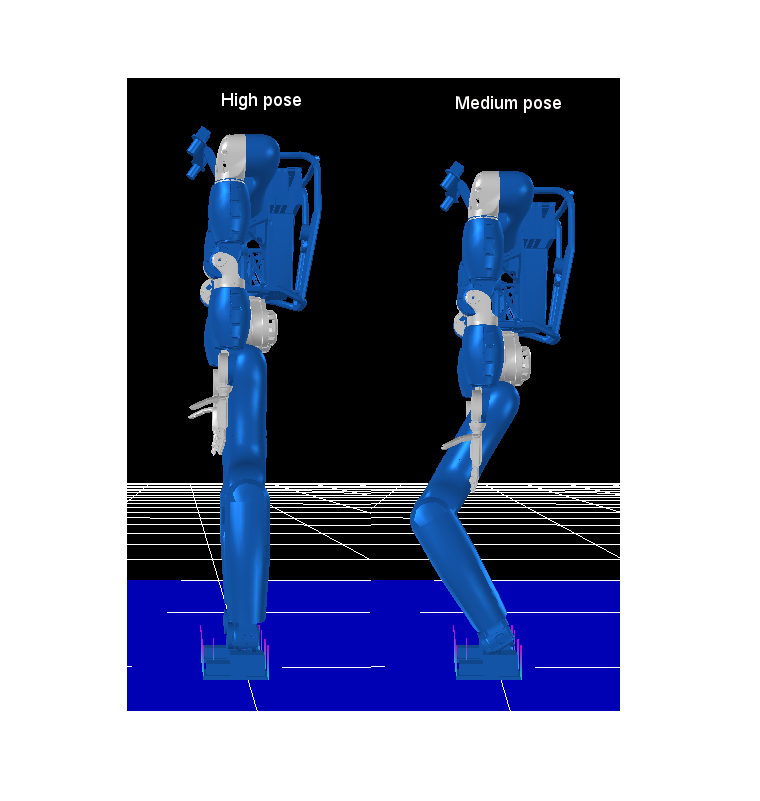
\includegraphics[width=0.7\textwidth,height=0.4\textheight]{Bilder/toro_high_medium.png}
	\caption{Snapshots of two different pose of \emph{Toro} in OpenHRP3 simulation}
	\label{fig:toro_sim_high_low}
\end{figure}
\begin{figure}
	\centering
	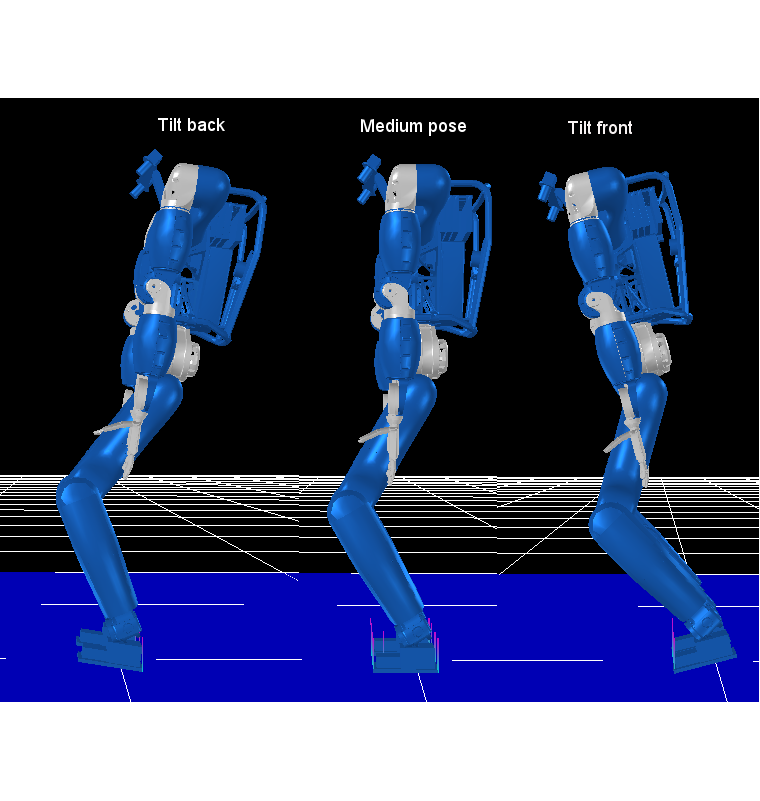
\includegraphics[width=0.7\textwidth, height=0.4\textheight]{Bilder/toro_tiltphase.png}
	\caption{Snapshots of tilting phase of \emph{Toro} in simulation}
	\label{fig:toro_tiltphase}
\end{figure}

\paragraph{Tilting phase:} After a few seconds an external force is applied to the robot so that it starts to tilt around an edge. After the robot has tilted few degrees the external force is removed,as a result the robot goes back to the medium pose due to inertia of the upper body. The robot stores the energy when the force is applied, it is not completely dissipated when it comes back to the medium pose. Inorder to dissipate the stored energy, it tilts in the other direction and then move back due to inertia. This cycle goes on until the robot dissipates all its stored energy. After the energy is dissipated the robot stays in the medium pose.
\paragraph{Final phase:} After the tilting phase is complete the robot is commanded to move back to the high pose.

The simulations and estimation are made with an integration time step of $\Delta t=1ms$. Zero mean Gaussian noises $w$ and $v$ are added to the inputs and measurements.
\begin{table}[H]
    \centering
    \begin{tabular}{|c|c|}
    \hline
    Name of the sensor &Noise variance \\ \hline
    \textbf{Input noise} &\hspace{2mm}\\
    FTS $W_r,W_l$ & $1 \cdot {10}^{-2}$ \\ 
    Torques $\tau$ & $1 \cdot {10}^{-4}$\\    \hline
    \textbf{Measurement noise} &\hspace{2mm}\\
    Joint angles $q(rad)$ &$1\cdot{10}^{-6}$ \\ 
    Joint velocities $\dot q(rad/s)$ &$1\cdot{10}^{-4}$ \\
    Acceleration $\dot v^b(m/s^2)$ &$1\cdot{10}^{-2}$ \\ 
    Angular velocity $\omega^b(rad/s)$ &$1\cdot{10}^{-4}$ \\ \hline
    \end{tabular}
    \caption{Variance of simulated noises}
    \label{tab:toro_var}
\end{table}

The values of the process and measuremt covariance matrices $Q$ and $R$ are set with the variance of the noises from Table \ref{tab:toro_var}. They are 
$$  \begin{aligned}
         Q &= diag([1\cdot{10}^{-2} \textbf{1}_{12,1}; 1\cdot{10}^{-4} \textbf{1}_{25,1}])  \\
         R &= diag([1\cdot{10}^{-6} \textbf{1}_{25,1}; 1\cdot{10}^{-4}\textbf{1}_{25,1}; 1\cdot{10}^{-2}\textbf{1}_{3,1};1\cdot{10}^{-4}\textbf{1}_{3,1}; 1\cdot{10}^{-12}\textbf{1}_{36,1} ]),
     \end{aligned}$$
where $\textbf{1}_{r,c}$ is the matrix of dimensions $r \times c$ with all the elements as 1 [Appendix \ref{sec:symbols}] and $diag(x)$ is a diagonal matrix where the main diagonal entries are the elements of vector $x$. 
The initial values of the system $x_0$ and estimator $\hat x_0$ are
$$ \begin{aligned} x_0 &= [0,0,1.164,\textbf{0}_{1,59}]^T \\ \hat x_0 &= \textbf{0}_{62,1}, \end{aligned} $$  where $\textbf{0}_{62,1}$ is the zero matrix of dimensions $62 \times 1$ [Appendix \ref{sec:symbols}].
The initial value of the covariance matrix $P_0$ is $$ P_0 = I_{62},$$ where $I_{62}$ respresents the identity matrix of dimensions $62\times62$. 

\subsubsection{Observation}
\begin{figure}
    \centering
    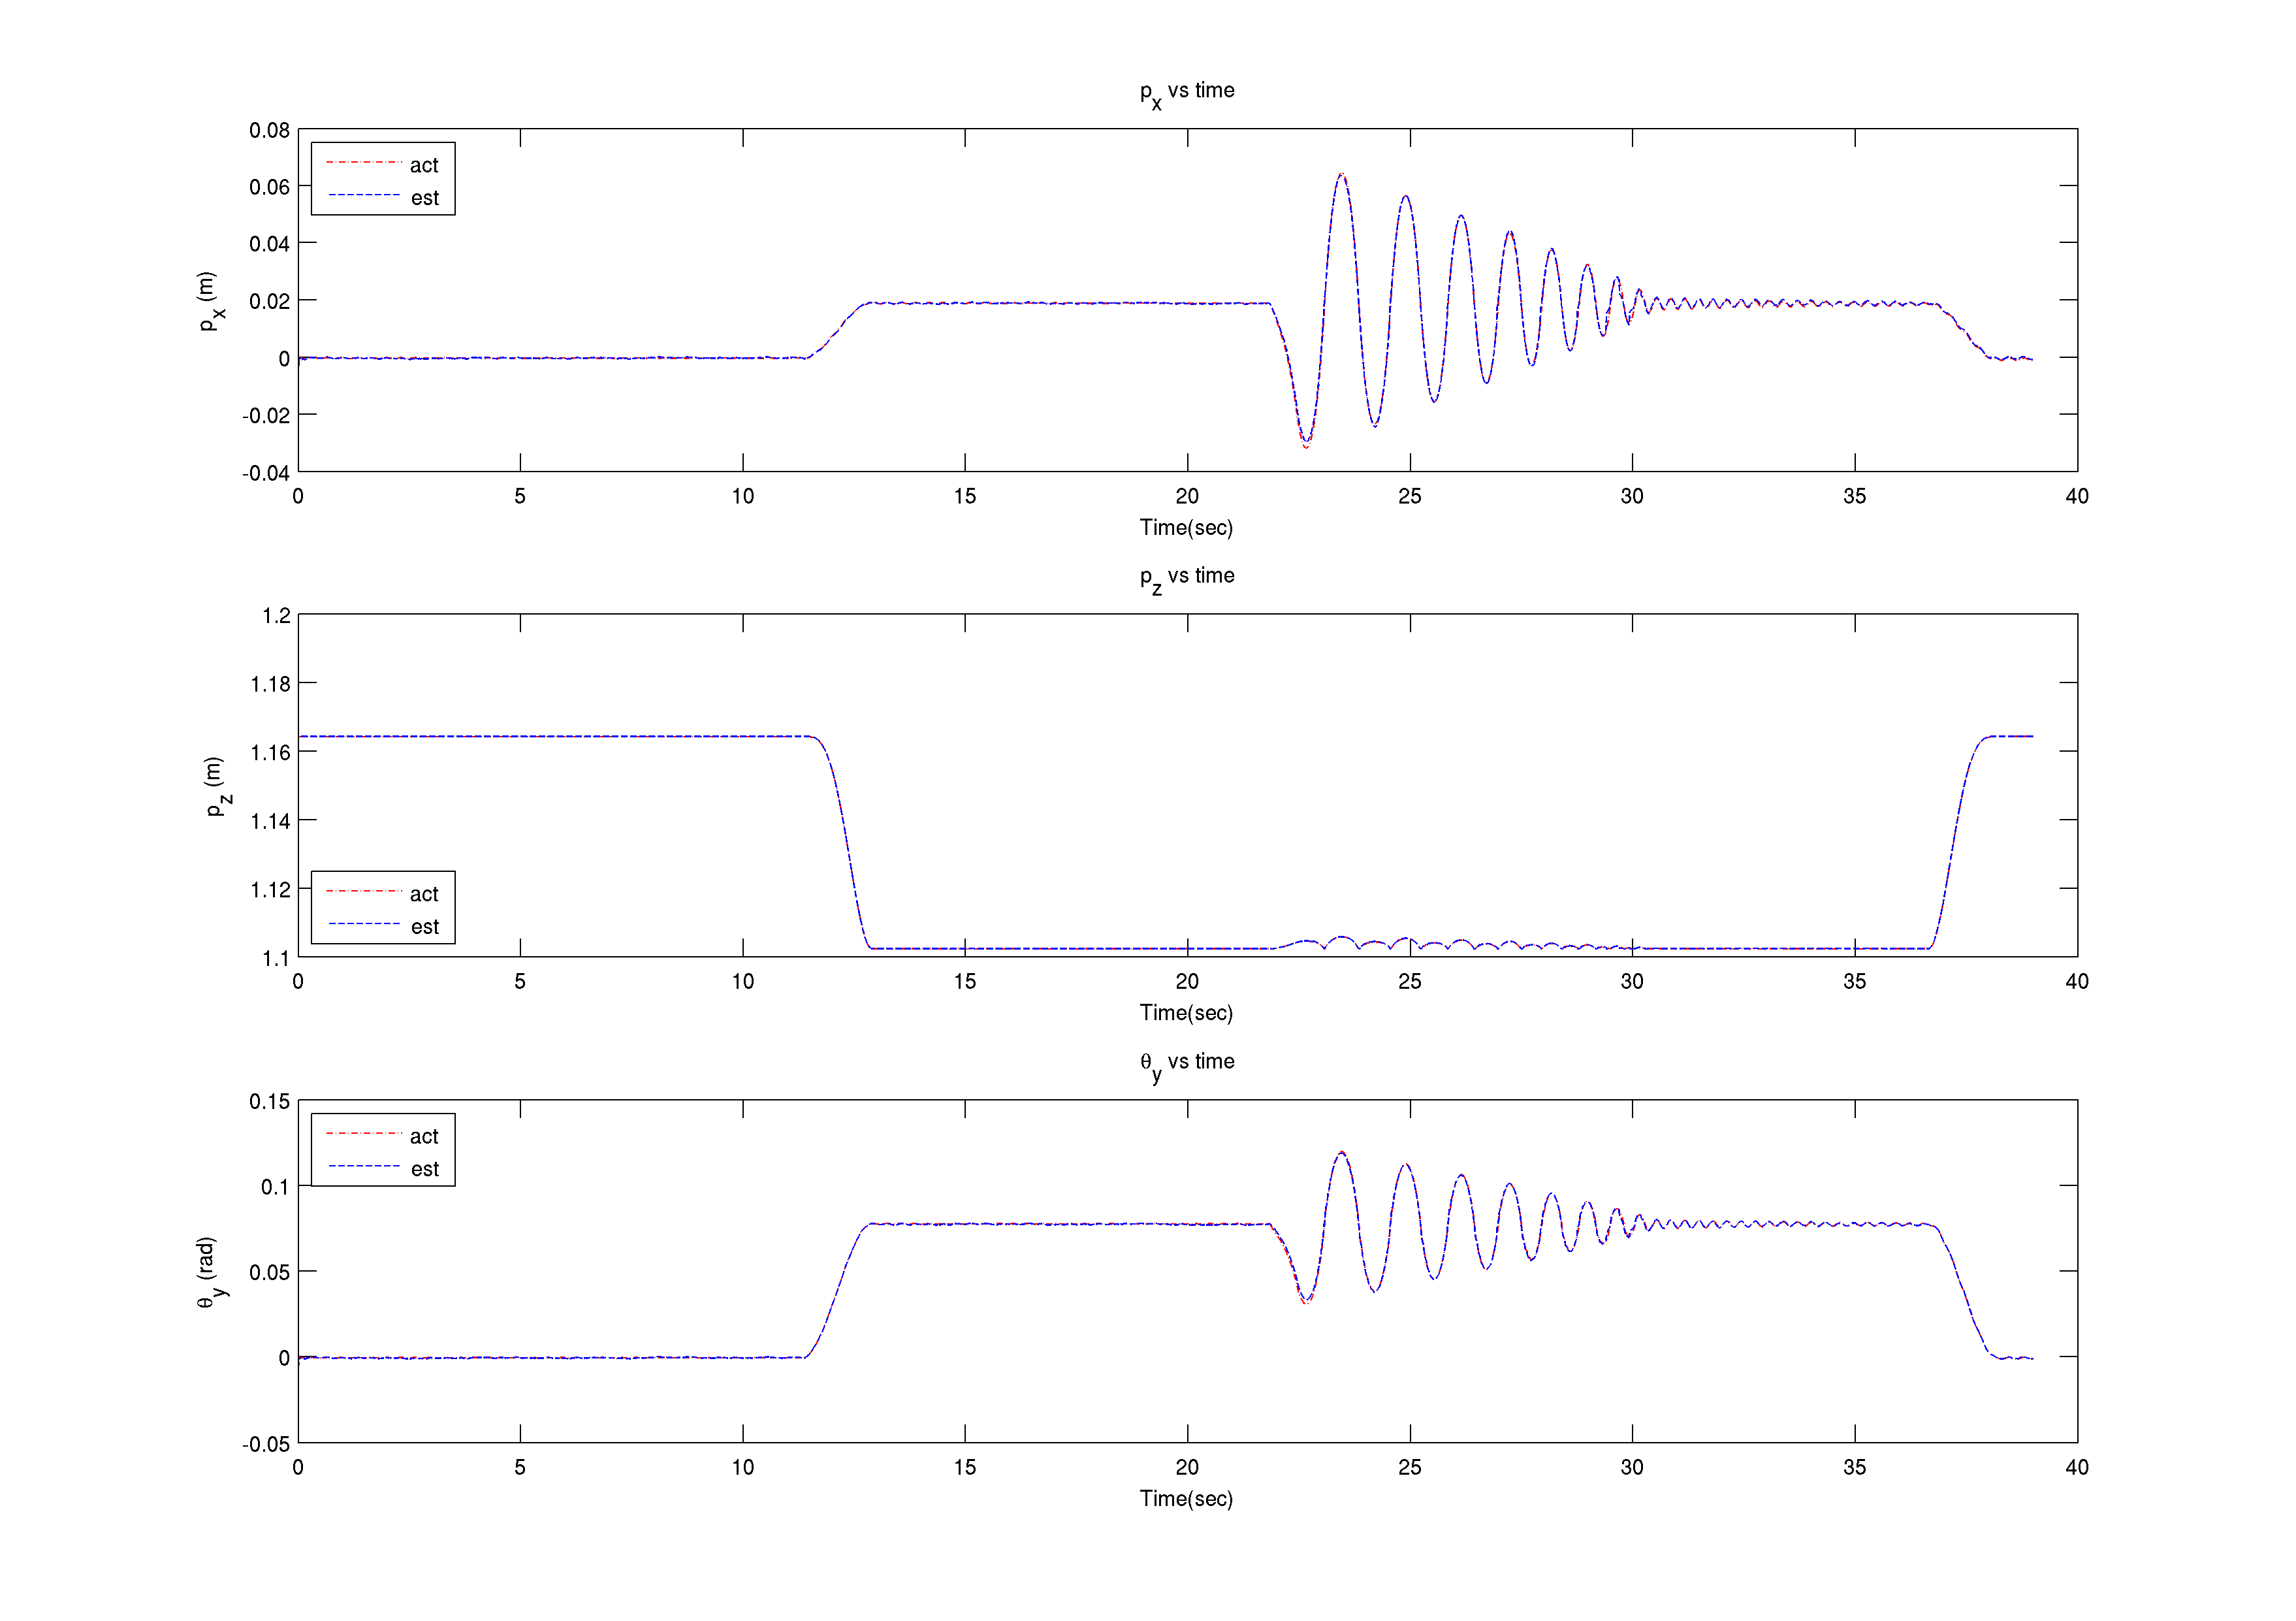
\includegraphics[trim=25mm 10mm 25mm 10mm,clip,scale=0.55]{Bilder/plots/toro/toro_pos.png}
    \caption{Actual and estimated values of $p_x,p_z$ and $\theta_y$}
    \label{fig:toro_plotpos}
\end{figure}
\begin{figure}
    \centering
    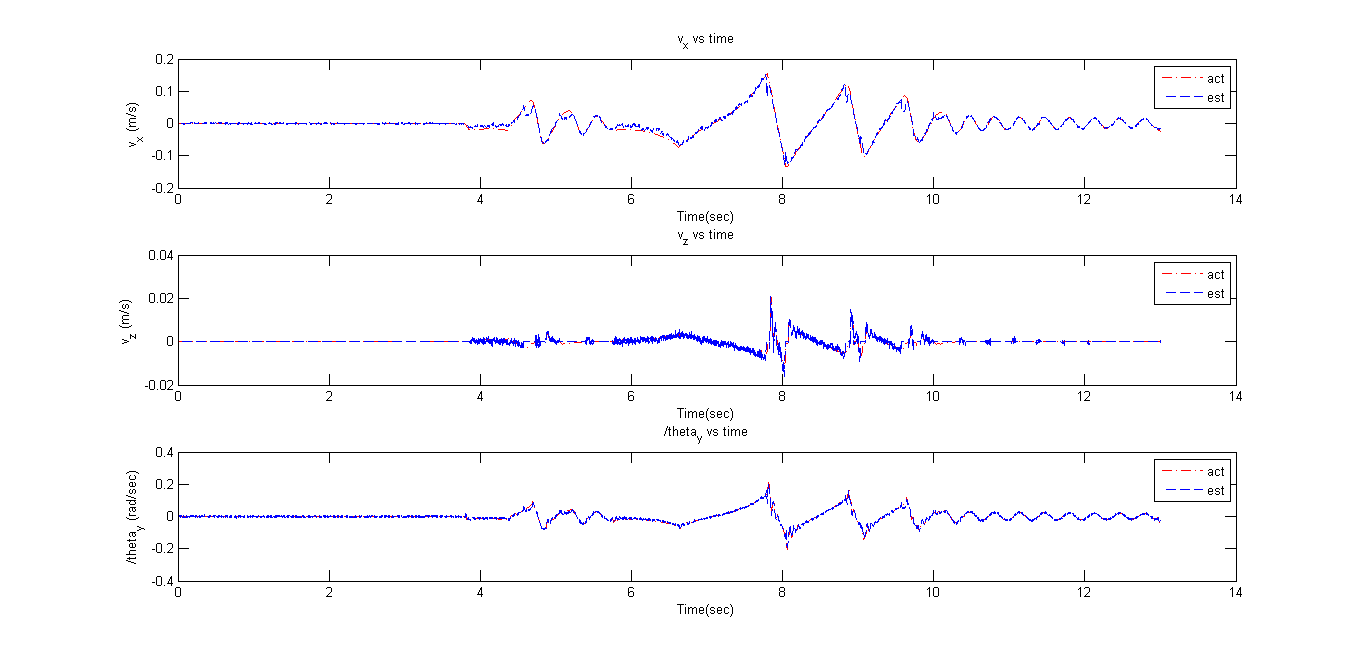
\includegraphics[trim=25mm 10mm 25mm 10mm,clip,scale=0.55]{Bilder/plots/toro/toro_vel.png}
    \caption{Actual and estimated values of $v_x,v_z$ and $\omega_y$}
    \label{fig:toro_plotvel}
\end{figure}

The robot tilts about the front and back edges of the foot. In other words it rotates about the $Y-axis$ of the spatial frame (world frame). A rotation of $\theta_y$ around $Y-axis$ will results in translation motions $p_x$ and $p_z$ along $X$ and $z$ axes. These three quantities are plotted in Figure \ref{fig:toro_plotpos}. The velocities of these quantities $\omega_y,v_x,v_z$ are plotted in Figure \ref{fig:toro_plotvel}.

In the the Figures \ref{fig:toro_plotpos} and \ref{fig:toro_plotvel} the time interval between $0-22s$ denotes the \emph{initial phase}, $22s-35s$ denotes the \emph{tilting phase} and $35s-39s$ denotes the \emph{final phase}. We can see in the above figures that, the estimates converges quickly to the actual states. 
\begin{table}
    \centering
    \begin{tabular}{|c|c|}
    \hline
    Estimates &RMSE \\ \hline
    $\hat p_x$ &0.0005 $m$\\
    $\hat p_y$ &0.0001 $m$\\
    $\hat p_z$ &0.0001 $m$\\
    $\hat\theta_x$ &0.0001 $rad$\\
    $\hat\theta_y$ &0.0006 $rad$\\
    $\hat\theta_z$ &0.0001 $rad$\\ \hline
    \end{tabular} \hspace{1cm}
    \begin{tabular}{|c|c|}
    \hline
    Estimates &RMSE \\ \hline
    $\hat v_x$ &0.0083 $m/s$\\
    $\hat v_y$ &0.0017 $m/s$\\
    $\hat v_z$ &0.0040 $m/s$\\
    $\hat\omega_x$ &0.0013 $rad/s$\\
    $\hat\omega_y$ &0.0042 $rad/s$\\
    $\hat\omega_z$ &0.0060 $rad/s$\\ \hline
    \end{tabular}
    \caption{RMSE values of the position and velocity estimates of the floating base}
    \label{tab:toro_rmse}
\end{table}

The RMSE values of the estimates in Table \ref{tab:toro_rmse} are small. This shows that EKF has a good performance for the given system model. The joint angles $ \hat q \in \Re^{25}$ and velocities $\hat \dot q \in \Re^{25}$ are also well estimated by the EKF. Since we focus on estimating the motion parameters of floating base, the joint's motion parameters are not discussed.

The time taken for 10 seconds of simulation of the EKF is $1290$ seconds. For each integration time step ($\Delta t = 0.001 s$) the EKF requires $0.129 s$ in real time for its execution. The high computation time is caused by the rigid body algorithm which has an execution time of $0.06s$. This algorithm is executed two times per time step.
$$ \text{Time take for the execution of rigid body algorithm } = 2 \times 0.06 = 0.12 s.$$ This is approximately the execution time of the EKF for one time step.

\subsection{Conclusion}
 With the multibody dynamic model of \emph{Toro} it is possible to estimate more than the under-actuated motion parameters. For example the joint velocity $\dot{q}$ can also be estimated. Although we have an advantage of estimating more motion parameters ($q, \dot{q}$), the main drawback is the computation time. A lot of effort is needed to setup the Jacobian matrices $A$ and $C$ for \emph{Toro} model. 
